%!TEX root = ../../report.tex
\chapter{Mechatronic design} % (fold)
\label{cha:design}
The results of the conceptual studies conducted in chapter \ref{cha:analysis} laid the goals and criteria to lead the design process of the first prototype of RuBi.
The actual implementation of these ideas in the fields of electronics, mechanics and software is described here.
When designing from a holistic point of view, these three areas combined give a positive synergy which is the burden of this chapter.
The first of the three sections starts with the design of the electronic hardware: from the selection of the motors based on \ref{sec:joints} and \ref{cha:mathematical_model} to the expansion interfaces installed in order to reduce the weight and finally the sensory feedback system.
It follows the mechanical design of the limbs components, in which the constraints defined in \ref{sec:dimensions} and \ref{sec:physical_properties} are applied, together with the structural and production-oriented calculations required.
It concludes with a presentation of the CAD design process carried out, in which a comprise between the components ideal capabilities and the current production capacity in this project has been tried to be reached.
In the last section, devoted to the software-related development except for the simulation environment, the architecture implemented for the robot control system is presented.

%!TEX root = ../../../report.tex
\section{Electronics} % (fold)
\label{sec:electronics}

%!TEX root = ../../../../report.tex

\subsection{The electric actuators} % (fold)
\label{sub:electric_actuators}
In chapter \ref{cha:mathematical_model}, the necessary characteristics of the actuators have been calculated.
In this section, the resulting theoretical requirements are used to select the final motor $+$ gearbox combination utilized.
All the documentation regarding the control of the actuators software-wise is to be found in section \ref{sec:software}.

\subsubsection{Flat BLDC Maxon motors} % (fold)
\label{ssub:the_bldc_motors}
It must be mentioned at this point that the actuators and their interface were assumed at the beginning of the project to be a very hard constraint in the design from an economic point of view. 
This means that the conception of the robot structure has been influenced by this criteria towards the adaption of the final prototype characteristics (such as final size or mass) to the application range of the available motors at our disposal.
This fact has converted the design in an iterative process of optimization whose final result is a robot that matches the available actuators and not the other way around, as it should be in theory.
In the view of the this, the brushless DC motor $+$ gearbox present in the Locokit robot construction kit, introduced in \cite{locokit} are used in the RuBi prototype.

The flat motors model is 339260 from Maxon motor, whose datasheet can be found in \cite{maxon_motor}, and the planetary gearhead is the number 143976 in datasheet \cite{maxon_gear}.
The electromechanical constants of the motors, together with its nominal supply values or the output power and torque of both the motor and the gearbox can be found in these documents. 
However, the electronics of the motors are designed to constantly overdrive them at $24V$, which has been taken into account when calculating their output.
Furthermore, each motor counts three hall effect sensors able to provide accurate relative position measurements.
% subsubsection the_bldc_motors (end)


\subsubsection{BLDC motor boards} % (fold)
\label{ssub:bldc_motor_boards}
Each BLDC motor in the Locokit comes with a motor board able to control it, designed for 24V and 48W.
They consist of a 48MHz ARM7 processor for time critical control and motor commutation, as stated in \cite{locokit-electronics}, together with 4 general purpose I/O inputs for local sensor interface.
Furthermore, they have two available 8-pin interfaces for the motors, one of them with a standard flex connector used in most of Maxon flat motors.

% subsubsection bldc_motor_boards (end)

\subsubsection{Extension PCBs} % (fold)
\label{ssub:extension_pcbs}
Following the idea of reducing weight and inertias in the structure as explained in chapter \ref{cha:analysis}, it was decided to place all the electronics off-board.
In order to extend the existing motor flex interfaces, a simple extension PCB was manufactured for each device.
The boards have been designed with Eagle following the requirements of current when sizing the width of the paths given by the supplier.
The design lacks of vias which reduces the complexity and facilitates the manufacturing.
The board for the left leg, whose schematic can be seen in \ref{fig:pcb1}\footnote{For the right leg the schematic has been mirrored}, contains a flex connector, like the one originally found on the motor boards, mapped to an 8-pin Molex connector where the wiring to the BLDC board is connected.

\begin{figure}[ht]
	\centering
	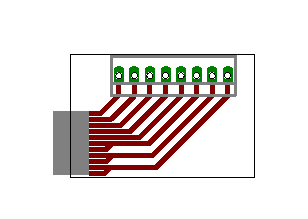
\includegraphics[width=0.5\textwidth]{figures/expansion_board.pdf}
	\caption{Left leg extension PCB schematic.}
	\label{fig:pcb1}
\end{figure}

% subsubsection extension_pcbs (end)


% subsection electric_actuators (end)
\subsection{Suitability of the motor model for the application} % (fold)
\label{sub:suitability_of_the_motor_model_for_the_application}
The algorithm designed to prove if the selected motor model fulfills the requirements of the application has been called Algorithm 1 and it is detailed in \ref{list:algorithm_1}.
The theoretical framework constructed in \ref{cha:mathematical_model} has been applied here to prove if the motors described above (without accounting on springs or indirect transmission) can be used to perform the vertical jumps described in \ref{sec:jumping_case}.
And if so, which height can be reached.

Algorithm 1:
\begin{enumerate}
\label{list:algorithm_1}
\item Manually set the values of $P_{3}(t_{0})$ and $P_{3}(t_{f})$ to use in equation \ref{eq:toe_trajectory}.
\item Compute the inverse kinematics model for the given trajectory equation. This yields as outputs $q_{j}(t)$, where j = 1,...,N being N = number of joints.
\item Compute forward kinematics to obtain $P_{j}(t)$.
\item Derive the two mentioned models and apply equation \ref{eq:angular_magnitudes} to obtain $\dot{P}_{j}$, $\ddot{P}_{j}$, $\omega_{j}$, $\omega_{j}$, $\dot{\omega}_{j}$,
\item Set $\Delta h$ and use the impulse equations \ref{eq:deltaV} and \ref{eq:impulse} to obtain a set of couple values of $(F_{i}, t_{i})$ as in Figure \ref{fig:f-t}.
\item For each couple until $(F_{min}, t_{max})$, obtained from \ref{eq:work}, compute the torques $\tau_{i,j}$ for each joint through \ref{eq:dynamics_eq1} and $\theta_{i,j}$ as in \ref{eq:joint_vel_2}\footnote{Eq. \ref{eq:joint_vel_2} introduced the assumption that the joint velocities are constant for simplicity}.
\item Compute the Torque/Speed curve for the motor + gearbox model as per equation \ref{eq:motor_curve}.
\item Plot the obtained pairs of values $(\dot{\theta}_{i,j}, \tau_{i,j})$ over the motor curve and analyze the results.
\end{enumerate}

\begin{equation}
\label{eq:joint_vel_2}
	\dot{\theta}_{i,j} =\frac{ \abs{ \theta_{j}(t_{f}) - \theta_{j}(t_{o}) } }{ t_{i} }
\end{equation}

\begin{equation}
\label{eq:motor_curve}
	\tau_{m} = \tau_{stall} - \omega_{m}\left(\frac{\tau_{stall}}{\omega_{n}}\right)
\end{equation}

\paragraph{Use case} % (fold)
\label{par:example_of_use}
As with any kind of DC motor, the goal is that the operation points lay under the torque/speed curve for a given application.
In this case, the operation point to study has been chosen to be the initial instant of the launch phase during the jump, given by $t_{0}=0s$, because it has been assumed to be the most requiring one of the whole jump cycle.
The input data for the test conducted with the algorithm can be seen in \ref{eq:input_a1}.

\begin{equation*}
\label{eq:input_a1}
\begin{aligned}[c]
P_{3}(t_{0}) &= \left[\!
				    \begin{array}{c}
				      0 \\
				      0.3508 \\
				      -\frac{\pi}{2}
				    \end{array}
				  \!\right]
\end{aligned}
\qquad
\begin{aligned}[c]
P_{3}(t_{f}) &= \left[\!
				    \begin{array}{c}
				      0 \\
				      L \\
				      0
				    \end{array}
				  \!\right]
\end{aligned}
\qquad
\begin{aligned}[c]
\Delta h &= 0.05 \\
\end{aligned}
\end{equation*}

The results can be seen in Figure \ref{fig:alg1_results} for a jumping leg.
It can be seen that, for the obtained $(\theta_{i,j}, \tau_{i,j})$ values for the given $\Delta h$, the closer they get to the theoretical $(F_{min}, t_{max})$, the more the application points approach the lower-left corner of the graph.
The aimed situation here is that in which the application points for the three motors lay under the motor curve, which occurs for values next to the couple $(4.1191N, 0.1700s)$

\begin{figure}[htb]
	\centering
	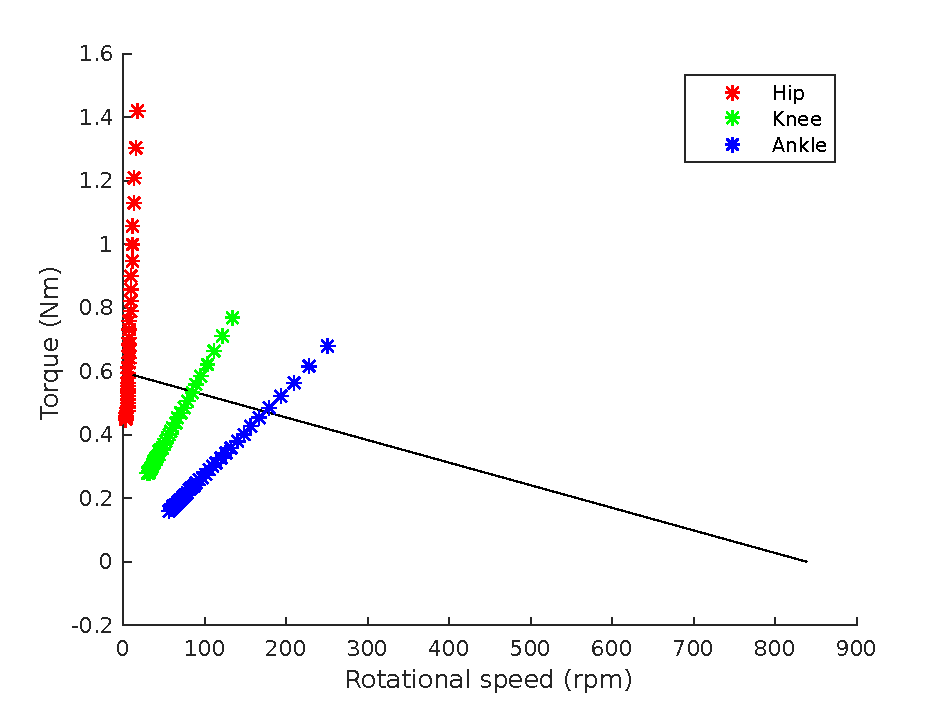
\includegraphics[width=0.9\textwidth]{figures/algorithm1.pdf}
	\caption{Results of Algorithm 1 for the given inputs (not all the $(\theta_{i,j}, \tau_{i,j})$ pairs are plotted).}
	\label{fig:alg1_results}
\end{figure}

\paragraph{The transmission on the hips} % (fold)
\label{par:the_hip_joint_gears}
The results from the presented algorithm helped notice that the presented motor model would not be able to accomplish the requirements of the application on the hip joints, due to its, in general, lower velocity and higher torque values.
Thus, the algorithm was used to approximate the required ratio of the gear system described in \ref{sub:gears}, used to adequate its output to the task.
The final ratio implemented and used for the results in \ref{fig:alg1_results} is $w=2$. 
However, it was calculated for the geometrical and inertial parameters of a different iteration than the last one, resulting in a non-optimal value for the final robot.
A repetition of the process yielded an optimal gear ratio of $w=1.2$, for which the best application points of the three motors would be closer to the motor line.

% paragraph the_hip_joint_gears (end)

The presented method does not aim at providing exact results since its based in several assumptions and simplifications from its basis.
It was conceived due to the necessity of assessing the utility of the existing actuators to the designed application.
Ideally, its results would have been tested by comparing them to the real data collected from the experimentation with the final prototype. 
However, the delay in some essential components of the robot prevented from testing and improving the model used for the algorithm, together with its validity.

% paragraph example_of_use (end)




% subsection suitability_of_the_motor_model_for_the_application (end)
%!TEX root = ../../../../report.tex

\subsection{Embedded electronics} % (fold)
\label{sub:locokit_electronics}
The Locokit main processor is a standard Gumstix Overo Air board with a 600MHz OMAP3, 512MB RAM and WiFi \cite{gumstix}.
It is mounted on a expansion board that provides interfaces as I2C, USB or GPIOs along with some on-board sensors not used here and the connection to the power board.
The power board was designed to allow a stable voltage of 24V and a maximum current of 10A with an efficiency of 90-95$\%$, as stated in \cite{locokit-electronics}.
It also makes available the connectors for the six-wire bus connection to the motor boards.
The communication between the main processor and each ARM7 in the motor boards is carried out through a system of common registers that are updated in every cycle of transfer, and for which each BLDC board only reads its assigned slots.
The addresses of these registers are given through the external switches on the bottom of every motor board.
The current configuration is given in table \ref{tab:motor_boards_addresses}.

\begin{table}
\begin{center}
\begin{tabular}{c | c}
  Controlled joint & Register address \\
  \hline
  Right hip & 7 \\
  Right knee & 11 \\
  Right ankle & 19 \\
  Left hip & 5 \\
  Left knee & 8\\
  Left ankle & 4 
\end{tabular}
\caption{Internal register addresses of motor boards}
\label{tab:motor_boards_addresses}
\end{center}
\end{table}

Each ARM7 reads the motor commands and writes the sensory feedback information on its register, reducing computation load in the main processor and simplifying the extension of the system with more motor boards to a simple connection.
As a result, the LocoKit electronics platform provides a reliable power supply and time critical control of actuators, an easily extensible and reconfigurable architecture, communication capabilities with external equipment and possibilities for sensory feedback handling.
All these features made it optimal for the expected requirements of the RuBi robot hardware, and led to its use on the project. 

%Add power requirements calculations?


% subsection locokit_electronics (end)
%!TEX root = ../../../../report.tex

\subsection{Sensory feedback} % (fold)
\label{sub:sensory_feedback}
As stated in the initial description of the project in \ref{sec:overall_description}, the first prototype of RuBi has been designed to provide the necessary capabilities to be controlled by an existing neural controller developed in \cite{dacbot1} and already tested in the DACbot robot.
The cited control algorithm requires as inputs the angular positions of all the joints in can actuate, besides ground contact signals from the feet for its reflex-based controller part.
All the documentation regarding the handling of the sensor readings software-wise is to be found in section \ref{sec:software}.


\subsubsection{Joint position information} % (fold)
\label{ssub:joint_position_feedback}
To provide the physical readings of the angular positions of the joints, the built-in hall sensors in the motors are utilized. 
Three wires transmit the hall effect sensors signals to the motor board for each joint, where they are written in the internal register and transferred to the main processor for its posterior treatment.
% subsubsection joint_position_feedback (end)

\subsubsection{Ground contact signal} % (fold)
\label{ssub:ground_contact_feedback}
One contact switch model Omron D2F-01F-T has been placed on the edge of the sole of each foot, under the heel in order to detect when the feet are standing on the ground. 
Their wiring has been extended to the main processor board, but the necessary pull-up resistors have not been implemented since the input pins on the processor could not be set up.
The mapping between the processor's GPIOS handlers and the physical pins on the board could not be found.
Therefore this last step is left as further work.
Alternatives to the use of the main board pins are discussed in chapter \ref{cha:discussion}, in case they cannot be used.
% subsubsection ground_contact_feedback (end)

% subsection sensory_feedback (end)

% section electronics (end)
%!TEX root = ../../../report.tex
\section{Mechanics} % (fold)
\label{sec:mechanics}
%!TEX root = ../../../../report.tex
\subsection{Pulleys and belts} % (fold)

\label{sub:pulleys_and_belts}
Section \ref{sec:joints} has been dedicated to analyze and define the kind of motor configuration and transmission system which is going to be used for each joint.
In the case of the knee and the ankle, the combination \textit{motor + gearbox + belt and pulleys} was selected, as explained before, following inertial-reduction criteria.
The transmission system designed to convey the motion from the motor shaft to the joint consists finally in the \textit{pulley+belt} presented here plus a torsional spring in series used to transfer the rotation movement from the joint pulley to the limb, as discussed in \ref{sub:compliance}.
As a result, an interface between the pulley and a spring holder was needed.
Hence, the design of the pulley itself has been studied in terms of two factors: \textit{precision and backlash reduction} and \textit{integration with the series torsional spring}.

\subsubsection{System backlash reduction} % (fold)
\label{ssub:precision_and_backlash_reduction}
All the pairs of pulleys are meant to have the same diameters since they are not planned to be used for torque-speed ratio modifications between actuators and joints. 
Thus, the final value of this dimension obeys only to other components dimensions constraints.
With that degree of freedom, the aim of the design process is to optimize the pulley in order to minimize their associated backlash, defined as the clearance between timing belt teeth and timing belt pulley grooves.
Despite the fact that the platform is going to be used mainly with adaptive controllers (e.g. ANN-based) and therefore the mechanical optimization is not a priority, the reduction of mechanical uncertainties is always sought.

After analyzing the current solutions in the market, several non-backlash solutions were found.
The optimal one seemed to be the Gates GT3 Synchronous Belts\footnote{http://www.gates.com/products/industrial/industrial-belts/synchronous-belts/powergrip-gt3-belts}, able to fulfill the requirements of the presented application.
The withdrawals of this option were the time constraints for ordering such parts and the increase in the final price of the product. 
But also, the integration with the series torsional spring.
% subsubsection precision_and_backlash_reduction (end)

\subsubsection{Integration of the pulleys with the series torsional springs} % (fold)
\label{ssub:integration_with_the_series_rotational}
An alternative solution was to design and manufacture the pulley, which would allow a complete control of the design and manufacturing process, thus yielding the possibility of integrating in a single part the pulley and the spring holder.
At first, the GT3 design from Gates was intended to be utilized as a model.
However its design, which is described in U.S. Patent Number 4,515,577, is patented and not open to the public.
As an alternative, the ISO 13050:2014 \cite{ISO13050}, following the type T, was used to create the model of the customized pulley.
This choice was based on its focus in efficiency and reduction of backlash, together with its optimality for accurate movements with high torques and low speeds, as the intended application here.
The physical properties of the pulleys as the number of teeth, width, etc... were selected according to the ISO 5295:1987 \cite{ISO5295}, and as mentioned before, with the view on their manufacturability.

The interface between the described pulley and the limb was created as a torsional spring leg holder attached to the pulley's side.
An equivalent piece was placed on the joint, turned $90\degree$ for holding the other leg of the spring, which is meant to be coiled around the axis of the joint.
Based on the two ISO norms cited before and after some iterations based on experimental tests, the pulley T2,5 of 19 teeth gave the expected behavior.
In Figure \ref{fig:motor_pulley} a detail of the final pulleys can be seen.
Figure \ref{fig:serial_spring_pulley} shows the pulley side of the series spring interface.
% subsubsection integration_with_the_series_rotational (end)

\subsubsection{Belts selection} % (fold)
\label{ssub:belts}
From \ref{ssub:integration_with_the_series_rotational} a system pulleys-belt using T2,5 teeth profile was selected.
For the implementation of the belt system, an open belt whose initial tension can be adjusted with a zip-tie is chosen.
This allows to adjust the tension at any moment without the need of further tools.
Besides, it facilitates the system maintenance.
However, no studies were conducted on the right amount of tension to apply to the belts. 
The complex dependency of the tension values on the application requirements led to their empirical adjustment as the most suitable option.
% subsubsection belts (end)

% subsection pulleys_and_belts (end)
%!TEX root = ../../../../report.tex
\subsection{Gears} % (fold)
\label{sub:gears}
When sizing the motors in \ref{cha:mathematical_model}, the same kind of motor for all the the joints was chosen reducing then the number of unique parts and increasing the modularity.
However, a reduction of $2:1$ was found to be needed for the hip joints during the calculations carried out in \ref{sub:suitability_of_the_motor_model_for_the_application}.
As defined in the analysis chapter \ref{cha:analysis}, the hip will be designed without any passive actuator and the motor will be as close as possible to the joint, which made a geared transmission the most appropriated option.

The gears have been optimized based on a trade-off between manufacturability and performance.
An small teeth size was sought in order to reduce the backlash and assuring that there are always teeth in contact.
The size of the teeth has been defined by the smaller precision of the 3D printer in which they were printed.
The gears have been designed with the \textit{Coarse Pitch Involute 20 deg} standard due to its easy manufacturability.
Despite a \textit{herringbone} gear was considered, the simple \textit{spur} was chosen since it facilitated the assembly and could be adapted to unpredicted problems in the manufacturing and assembly processes. 
In the Figure \ref{fig:teeth_detail}, a detail of the teeth is shown.

\begin{figure}[ht!]
  \centering
  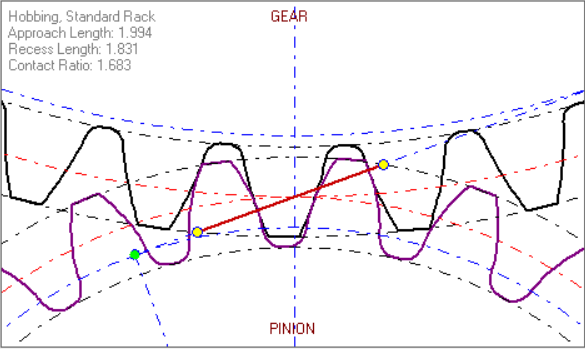
\includegraphics[width=0.6\textwidth]{figures/hip_gears}
  \caption{Teeth detail from pinion and gear.}
  \label{fig:teeth_detail}
\end{figure}

There was not a FEM or stress analysis and the experimental method was preferred due to the current unpredictable mechanical efforts of the 3D printed parts.
In the appendix \ref{app:hip_gears}, all the properties of the gears are to be found.

% subsection gears (end)
%!TEX root = ../../../../report.tex
\subsection{Landing impact force} % (fold)
\label{sub:impact_force}
The assessment of the desired mechanical characteristics of some of the components in the limbs requires the calculation of the internal forces they will be subjected to during the motion.
This process would normally entail the creation of an impact model for the feet and the ground, which due to its complexity has been left as further work.
To approximate the output of this model, the calculations of the energy transferred to a landing leg in collision with the ground have been carried out using the model of falling object hitting the ground.
The assumptions made for the scenario are listed in \ref{list:impact_model}.

\begin{enumerate}
\label{list:impact_model}
	\item No bouncing or slippering 
	\item No losses of energy between states
	\item No compliance on the leg
	\item No deformation on the ground surface
	\item All the initial potential energy before the fall is dissipated in the impact 
\end{enumerate}

This energy in then transmitted from the first contact point, the footprint, to the rest of the system, causing stresses that must be absorbed.
The components of the system must receive that energy under a controlled behavior - elastic deformations- ensuring a longer service life of the materials.
Thus, some input parameters to calculate the impact force are assumed.
From this force all the consecutive components in the deformation chain will be sized.
Despite the deformation is of the whole system, the security coefficient assumed in here is going to be the calculation of all the components for that maximum force.

From the formula of the mechanical energy:
\begin{equation}
  E_{mechanical} = m g \Delta h + \frac{1}{2} m v^{2}
\end{equation}

For a free falling object in the defined scenario, it is assumed that all the potential energy on the first instant is transferred to the crash without intermediary loses.
This energy is then translated into force by supposing a deformation of the whole body as expressed in the equation \ref{eq:impact_force}.

\begin{equation}
\label{eq:impact_force}
  F_{impact} = \frac{m g \Delta h}{d_{impact\_displacement}} = 294.40 N 
\end{equation}

The equation \ref{eq:impact_force} gives the force for sizing all the components.
Based on the input parameters defined in the appendix \ref{app:profile_selection} which are shown in the table \ref{tab:input_parameter_impact_force}.
\begin{table}
\begin{center}
\begin{tabular}{c | c}
  Parameter & Value \\
  \hline
  Total mass [kg] & 1.5 \\
  Jumping height [m] & 0.1 \\
  Impact displacement [m] & 0.005
\end{tabular}
\caption{Input parameters for calculating the impact force}
\label{tab:input_parameter_impact_force}
\end{center}
\end{table}

%!TEX root = ../../../../report.tex
\subsection{Limbs profile} % (fold)
\label{sub:limb_profile}
Based on the requirements of weight and its desired distribution defined in the structural analysis of the robot, in the joints study in \ref{sec:joints} it was decided to place the actuators as further up in the limbs as possible.
This left the functionality of the limb as the frame to hold the joint components on both ends plus the actuator, also working as a placement for the wiring.
Thus, a lightweight section that satisfies the conditions of deformation and stress was needed.
Carbon fiber seemed to be an ideal material to achieve these conditions of weight and stress, so a generic quantitative analysis was carried out to calculate the optimal profile with this material between the ones offered by the available provider.
The provider was chosen due to previous experiences that the Mærsk Mc-Kinney Møller Institute had with carbon fiber orders.

The section profile offered\footnote{http://www.easycomposites.co.uk/\#!/cured-carbon-fibre-products/} are: \textit{Rod}, \textit{Tube}, \textit{Box}. The \textit{Stripe} and the \textit{Angle} were discarded due to their asymmetrical geometry that would lead to less predictable scenarios.
The study case is show in the Figure \ref{fig:impact_decomposition}, where the impact force could be decomposed into pure bending and pure compression effort components.
Since the resistance of the carbon fiber in pure compression is greater than in under a bending effort, only this last case has been studied because of it is the most possible cause of failure.
This study does not completely model the behavior in real life of the limb due to the fact that carbon fiber is not an isomorphic material.
However, the high security factor taken into account is expected to overcome this.

\begin{figure}[ht!]
  \centering
  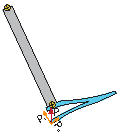
\includegraphics[width=.3\textwidth]{figures/impact_decomposition.pdf}
  \caption{Impact force decomposed.}
  \label{fig:impact_decomposition}
\end{figure}

\subsubsection{Profile study} % (fold)
\label{ssub:profile_study}
  The bending effort causes two types of problems: (1) the possible break in the supporting point and (2) the deformation suffered by the beam.
  The break might occur when the internal tensions created are over the ultimate effort in compression or tension of the selected material.
  This is modeled in equation \ref{eq:tension} for symmetric sections and when a single torque $M$ is being applied.
  \begin{equation}
  \label{eq:tension}
    \sigma _{compression} = \sigma _{tension} = \frac{M h_{CG}}{I_x}
  \end{equation}

  Meanwhile the deformation in the extreme can be calculated with the equation \ref{eq:deformation} if the case is simplified to the one depicted in the Figure \ref{fig:bending_case}.
  This is, when the leg is completely stretched to its limits, which is when it will be subjected to the biggest stresses.
  Thus, the leg can be analyzed as a simple straight beam attached to a fixed point with no degrees of freedom, to which a force $P$ (corresponding to $P_{b}$ in \ref{fig:impact_decomposition}) is being applied.

  \begin{figure}[ht!]
    \centering
    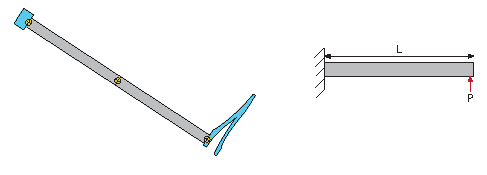
\includegraphics[width=\textwidth]{figures/bending_case.pdf}
    \caption{Simplified representation of the bending case.}
    \label{fig:bending_case}
  \end{figure}

  \begin{equation}
  \label{eq:deformation}
    y_L = \frac{P z^2}{6EI}(3L-z) = \frac{P L^2}{6EI}(2L) = \frac{P L^2}{3EI}
  \end{equation}


  For the selected profiles the equations that define the compression ($\sigma _{compression}$) and tension ($\sigma _{tension}$) efforts, along with the deformation in the direction of the applied force ($y_L$) are shown in the table \ref{tab:section_study}, being:

  \begin{enumerate}
    \item $h_{CG}$: height of the center of gravity of the semi-half section from the geometrical center of the section.
    \item $E$: Elastic module.
  \end{enumerate}

  \begin{table}[ht!]
  \centering
  \begin{tabular}{c|c|c|c|c}
    \textbf{Section} & \textbf{$I$} & \textbf{$h_{CG}$} & \textbf{$y_L$} & \textbf{$\sigma$} \\ \hline
    \raisebox{-.5\height}{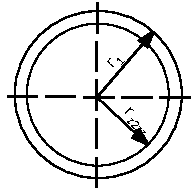
\includegraphics[width=0.25\linewidth]{figures/profile_cylinder.pdf}} & $\frac{\pi}{4} (r_2 ^4 - r_1 ^4)$ & $r_2$ & $\frac{4 P L^2}{3 E \pi(r_2 ^4 - r_1 ^4)}$ & ${\pi(r_2 ^4 - r_1 ^4)} M$ \\ \hline

    \raisebox{-.5\height}{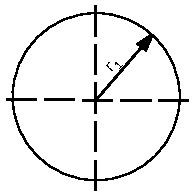
\includegraphics[width=0.25\linewidth]{figures/profile_tube.pdf}} & $\frac{\pi r_1 ^4}{4}$ & $r_1$ & $\frac{4 P L^2}{3 E \pi r_1 ^4}$ & $\frac{4}{\pi r_1 ^3} M$ \\ \hline

    \raisebox{-.5\height}{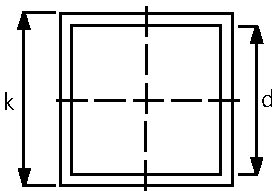
\includegraphics[width=0.33\linewidth]{figures/profile_squared.pdf}} & $\frac{1}{12} (d^4 - k^4)$ & $\frac{d}{2}$ & $\frac{4 P L^2}{E (d^4 - k^4)}$ & $\frac{6 d}{(d^4 - k^4)}$ \\ \hline
  \end{tabular}
  \caption{Stress and deformation analysis for the sections given.}
  \label{tab:section_study}
  \end{table}
% subsubsection profile_study (end)

\subsubsection{Torque calculation} % (fold)
\label{ssub:torque_calculation}
  For both the profile of the lower and the upper limbs, the torque generated by the impact force determined in the section \ref{sub:impact_force}, is calculated through equation \ref{eq:internal_torque}.
  The torque differs in the limbs due to the fact that the applied on the upper limb is computed with the distance from the foot to the hip while the other one is only from the foot to the knee:
  
  \begin{equation}
  \begin{aligned}
  \label{eq:internal_torque}
     M_{lower\ limb} = F \cdot l_{link(s)\ length}
  \end{aligned}
  \end{equation}
% subsubsection torque_calculation (end)

\subsubsection{Final limb parameters} % (fold)
\label{ssub:final_limb_parameters}
Using the criteria defined in sections \ref{sec:dimensions} and \ref{sec:physical_properties} for sizes and materials, the presented formulas have been applied to all the profiles of the offered by the provider.
The outputs of the iterative analyses in \ref{cha:design} and \ref{cha:mathematical_model} are shown in the table \ref{tab:limb_physical_properties}. 
This final data is the used for the current stress study.

The profiles have been analyzed calculating the torque from \ref{ssub:torque_calculation} and then applying the section \ref{ssub:profile_study} for each iteration.
The calculations of the last iteration are shown in the appendix \ref{app:profile_selection}.
These results have been then approved or discarded based on a \textit{maximum deformation} and \textit{ultimate tension} requirements, and are shown in the table \ref{tab:profile_selection}

\begin{table}[ht!]
\centering
\caption{Profile selection for each limb.}
\label{tab:profile_selection}
\begin{tabular}{c|c|c}
  \textbf{Limb} & \textbf{Section} & \textbf{Dimensions} \\ \hline
  Lower limb & Tube & 20 mm and 1 mm thickness \\ \hline
  Upper limb & Tube & 20 mm and 1 mm thickness 
\end{tabular}
\end{table}

% subsubsection profile_selection (end)



% subsection limb_profile (end) 
%!TEX root = ../../../../report.tex

\subsection{Ankle and knee joint mechanics} % (fold)
\label{sub:hip_and_knee_joint_mechanics}
Several mechanical configurations were sketched as the first step of the iterations in the mechanical design of the joints.
As previously explained, the hip joint turned out to have lower design constraints, since belt and compliance were not required, although the use of gears was a need.
However, for the knee and ankle joints, the need of integrated compliance and the torque transmission through a pulley yielded some restrictions that resulted in a final configuration as in \ref{fig:knee_joint}.

\begin{figure}[h]
  \centering
  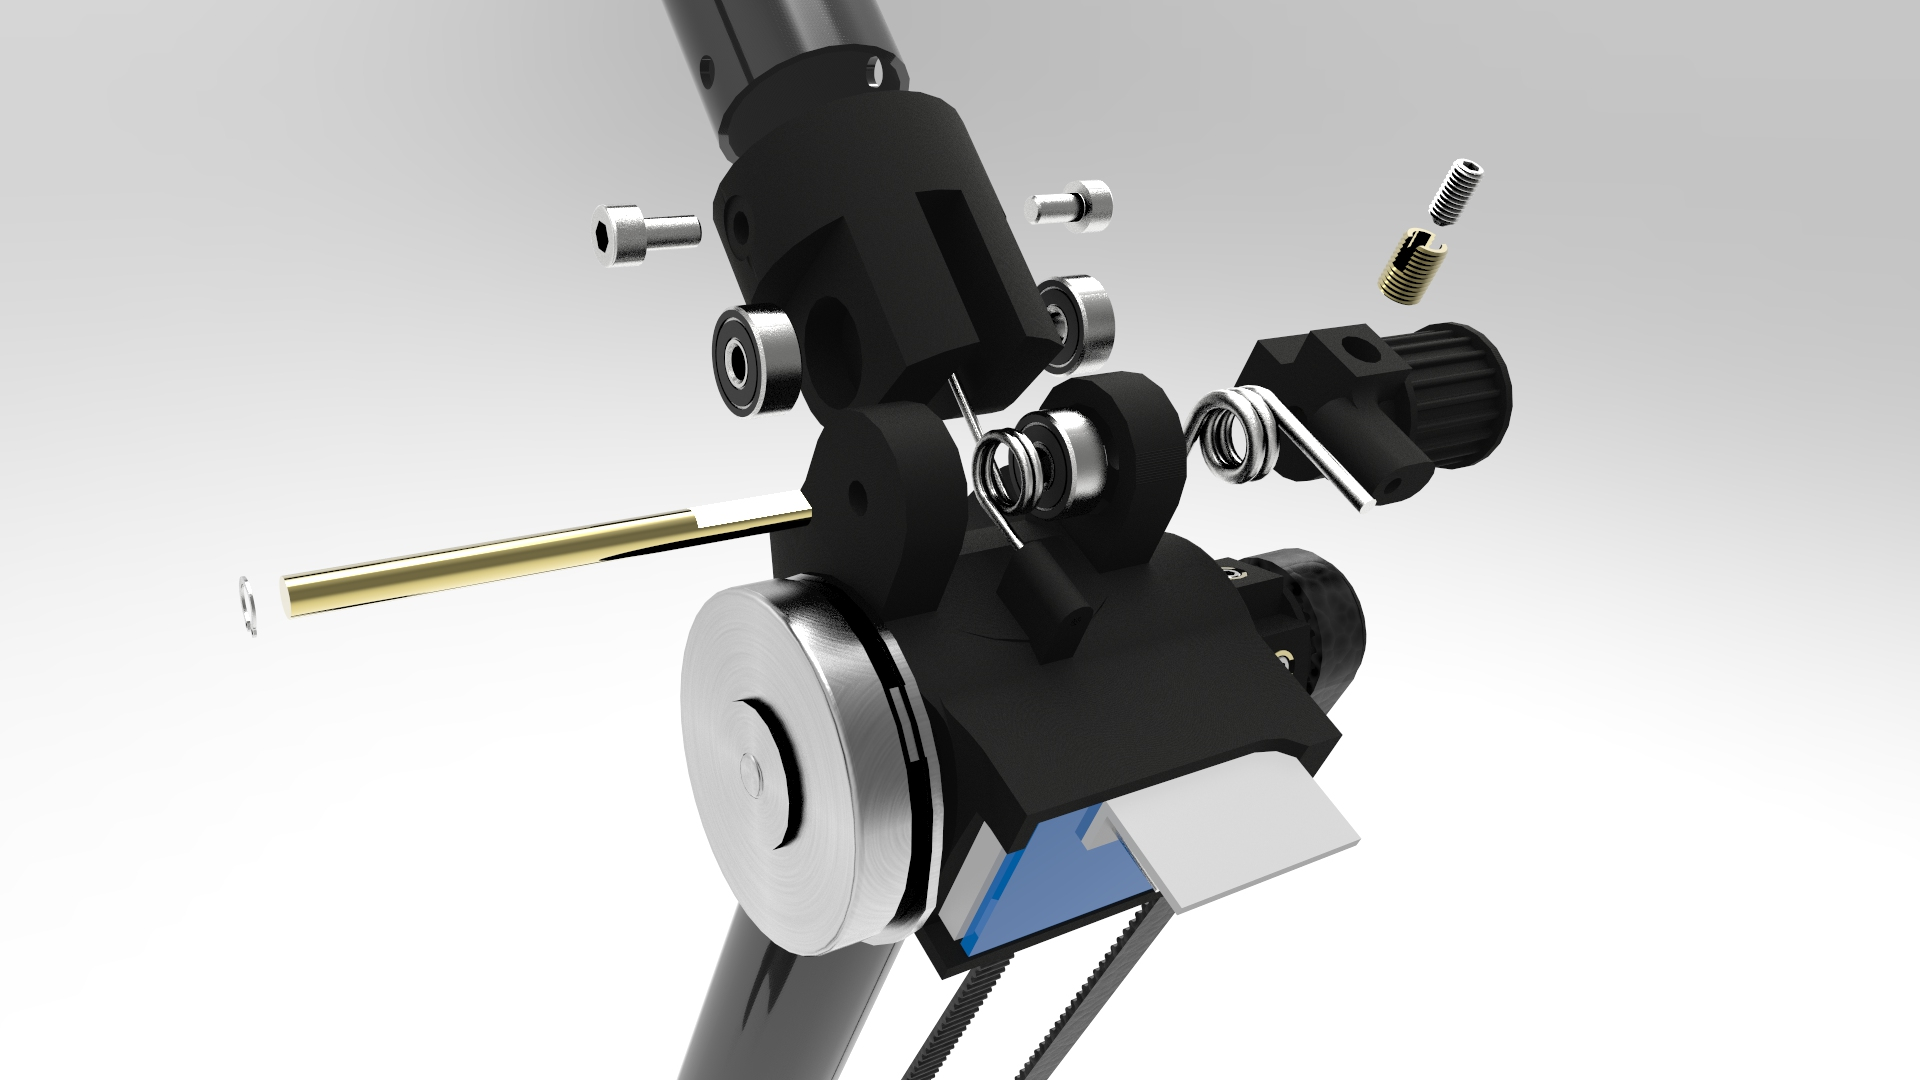
\includegraphics[width=\textwidth]{figures/legs_knee_deconstructed.jpg}
  \caption{Knee joint mechanical implementation}
  \label{fig:knee_joint}
\end{figure}

The configuration in \ref{fig:knee_joint} is equivalent for the ankles.
Therefore, four bearings, a rod and the interfaces for the springs are needed and thus, discussed below.

\subsubsection{Joints axes} % (fold)
\label{ssub:rods}
The characteristics of the rod used as axis of the angular motion of the joint are studied here.
It is also used, in the case of the knee and the ankle, as a support for the pulleys that transmit the power from the motor to the next link.
Three mechanical efforts bound its design:
\begin{enumerate}
  \item \textbf{Shear effort}: produced when an impact occurs and the internal efforts are transmitted through the rod between the two links that form the joint.
  \item \textbf{Bending effort}: caused by the perpendicular force created by belt in tension on the edge of the rod.
  \item \textbf{Torsion effort}: due to the pulley in the knee and the ankle. 
  This effort is negligible because zero-friction bearings are supposed.
\end{enumerate}

  \paragraph{Shear analysis} % (fold)
  \label{ssub:shear_analysis}
  The maximum shear stress is found in the diameter of the cylinder (y=0) and is:
  
  \noindent\begin{minipage}{0.2\textwidth}% adapt widths of minipages to your needs
  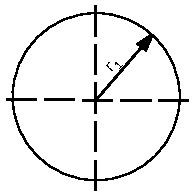
\includegraphics[width=\linewidth]{figures/profile_tube.pdf}
  \end{minipage}%
  \hfill%
  \begin{minipage}{0.8\textwidth}
    \begin{equation}
    \begin{aligned}
      \gamma_{yz} &= \frac{Q_y M_{x}^A*}{b(y) I_x} = \frac{Q}{r^2}\\
      M_{x}^{A_{y=0}} &= \frac{\pi r_1^2}{2} \\
      b(y=0) &= 2 r_1 \\
      I_x &= \frac{\pi r_1^4}{4}
      \end{aligned}
    \end{equation}
  \end{minipage}
  Given a tangent force Q, the shear stress can be calculated.
  If this is over the ultimate strength, the cylinder will break.
  % paragraph shear_analysis (end)

  \paragraph{Bending} % (fold)
  \label{ssub:bending}
  The bending analysis follows the one carried out in the section \ref{ssub:profile_study} for a cylinder.
  The equivalent force in this case is given by the tension of the belts, mainly the initial (though there are other tensions that appear when the belts moves for example).
  Due to feasibility reasons and the lack of the appropriate measurements devices, some experimental tests trying different tensions and axes where carried out giving good results with a 3 mm rod or more.
  % paragraph bending (end)

  \paragraph{Sizing} % (fold)
  \label{ssub:sizing}
  The studies above have been tested for different diameters of rod starting from the smallest size given by the provider and increasing until both conditions are satisfied, due to the requirements of weight reduction.
  In case of using steel as material, the ultimate strength is supposed to be 250 MPa \footnote{https://en.wikipedia.org/wiki/A36\_steel}.
  And for the case of a rod of 3 mm of diameter, both stress efforts are under the resulting restrictions.
  Thus, 3 mm rods were selected for both ankles and knees.
  % paragraph sizing (end)
% subsubsection rods (end)

\subsubsection{Bearings on the joints} % (fold)
\label{ssub:bearings}
The force calculated in section \ref{sub:impact_force} has been used for sizing the bearings of the knee and the ankle.
The bearing selected should be such that allowed dynamic loads of more than the impact force while being as small as possible to reduce additional weight on the frame.
Besides, their internal diameter is defined by the rod diameter calculated in section \ref{sub:rods}.

An estimation of nominal life of the bearing can be done from the Dynamic Load Rating (C), the Dynamic Equivalent Load (P) and the Life Rime Coefficient for a Ball Bearing (p) (being p=3 for balls bearings).
Equation \ref{eq:service_life_bearing} shows the nominal life of a ball bearing, which can be used in order to calculate the nominal life for a specific application.
It is also worth mentioning that the Dynamic Equivalent Load (P) is divided by the number of bearings in which the force is spread.
\begin{equation}
  \label{eq:service_life_bearing}
  L_{10} = \frac{10^{6}}{60 n} \left(\frac{C}{P}\right)^{p}
\end{equation}

The term $L$ is the service life of a bearing (in number of hours or rpm), in normal conditions of speed and load, in which the bearing is working until fail by fatigue. 
Whilst $L_{10}$ is based in a statistical model that is defined as the 90\% of the bearing of the same type will withstand those loads for a longer time.
% subsubsection bearings (end)

\subsubsection{Implementation of elastic actuation} % (fold)

\todo{Springs selection (shortly)}

\label{ssub:spring_integration}
In section \ref{sec:joints} the use of springs is justified in order to walk and run efficiently. 
An analysis of the different possibilities to include compliance in the robot is done in the same section, while Figure \ref{fig:compliance_series} shows the analyzed configurations and their advantages and disadvantages are further discussed.
The final design has been conceived to allow any of the four possible springs configurations shown in Figure \ref{fig:pasive_actuators} to be implemented in the knee and ankle joints.
This is possible by making a system that allows to put elastic components in series and parallel that are easily replaceable.
Furthermore, a big range of springs have been ordered for the reasons in explained in \ref{sec_springs}.
Any of the ordered springs can be placed due to the fact that the holes for inserting them have the diameter of the biggest one ordered plus a small clearance obtained from \ref{sub:arc_compensation}.

\paragraph{SEA configuration} % (fold)
\label{para:sea_configuration}

In the section commented above, it is also determined the use of rotational springs for both series and parallel passive actuators.
This gives a more constrained design that is later used as a feature.
For example, in the section \ref{sub:pulleys_and_belts} is explained how the the pulley is integrated in a part that has the task of both being the place to put the spring and being the pulley.
The Figure \ref{fig:serial_spring_pulley} shows this.
This design shows the implementation of the SEA configurations that can be adjusted by changing the physical properties of the spring.
% paragraph sea_configuration (end)

\paragraph{PEA configuration} % (fold)
\label{para:pea_configuration}

The parallel spring is implemented by adding a spring directly attached to both links of the joint.
The problem of the parallel passive actuators is the need of loading the spring for movements in which is maybe not appropriated.
As an example, the rest position of the parallel spring in the ankle could be placed when the foot is at 90 degrees with its consecutive link, so the robot can be stood up without applying any extra torque in the motors to keep balance.
This would mean though to do an extra effort against the spring when taking off.
In the same line of giving all the possibilities to the user with the compliance, a system that allows to change the rest position of the parallel spring has been implemented.
This consists of one arm of the torsional spring attached to one of the links of the joint while the other arm can be fastened in different relative angles.
The Figure \ref{fig:rotational_spring_rest_position} shows the transversal section of the joint component where the parallel spring can adopt different configurations. 

The above explained design allows to implement a PEA configuration on the joints by just adding a spring and using an overdimensioned spring for the transmission from the pulley that can act as a DD.

\begin{figure}[ht!]
  \centering
  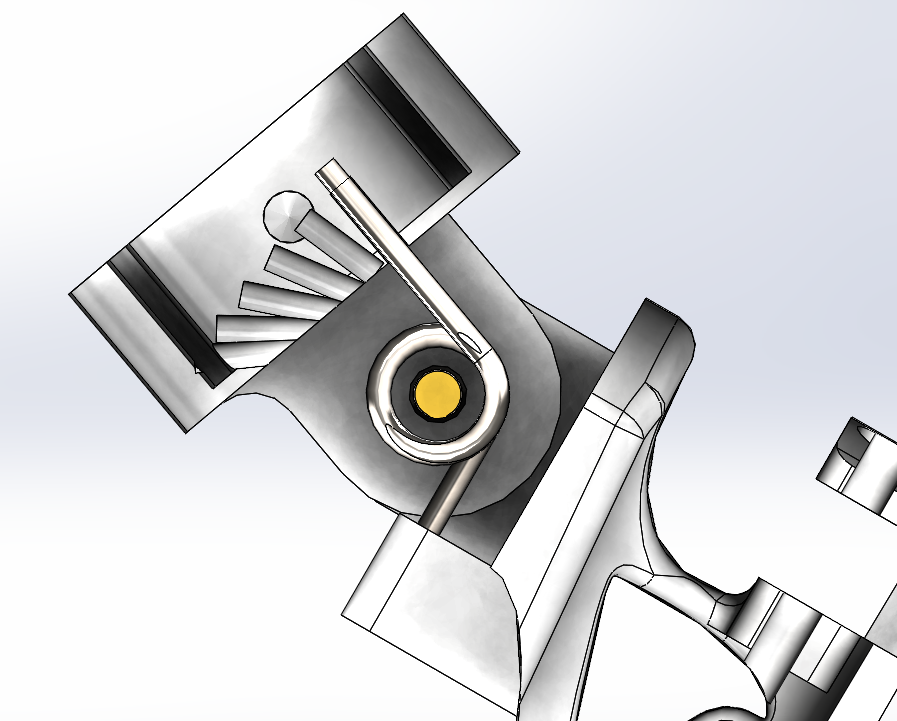
\includegraphics[width=0.75\textwidth]{figures/rotational_spring_rest_positions}
  \caption{Transversal section of the parallel spring resting positions in the left ankle.}
  \label{fig:rotational_spring_rest_position}
\end{figure}
% paragraph pea_configuration (end)

\paragraph{SEA + PEA configuration} % (fold)
\label{ssub:sea_pea_configuration}
The possibility of using both, SEA and PEA, configurations at the same time is offered.
This allows for the study of the SEA+PEA combination.
% paragraph sea_pea_configuration (end)

\paragraph{DD configuration } % (fold)
\label{ssub:dd_configuration}
Finally if no parallel spring is used and a spring stiff enough that does not add compliance to the system is placed in the SEA configuration, a DD transmission is achieved.
% paragraph dd_configuration (end)

% subsubsection spring_integration (end)

% subsection hip_and_knee_joint_mechanics (end)

%%!TEX root = ../../../../report.tex
\subsection{Rods} % (fold)
\label{sub:rods}
As explained in section \ref{sub:bearings}, it was decided to have two bearings per link (which gives four per joint) and a rod going through them.
This rod is then also used, in the case of the knee and the ankle, as a support for the pulleys that transmit the power from the motor to the next link.

Three mechanical efforts bound its design:
\begin{enumerate}
  \item \textbf{Shear strength}: in the case of the shear produced when an impact occurs and the rod of one link moves in the opposite direction than its relative in the consecutive link.
  \item \textbf{Resistance to bending}: due to the bending effort that the tension of the belt is constantly applying in the rod of the  knee and the ankle.
  \item \textbf{Torsion}: due to the pulley in the knee and the ankle. 
  This effort is negligible because zero-friction bearings are supposed.
\end{enumerate}

  \subsubsection{Shear analysis} % (fold)
  \label{ssub:shear_analysis}
  The maximum shear stress is found in the diameter of the cylinder (y=0) and is:
  
  \noindent\begin{minipage}{0.2\textwidth}% adapt widths of minipages to your needs
  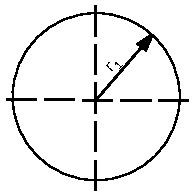
\includegraphics[width=\linewidth]{figures/profile_tube.pdf}
  \end{minipage}%
  \hfill%
  \begin{minipage}{0.8\textwidth}
    \begin{equation}
    \begin{aligned}
      \gamma_{yz} &= \frac{Q_y M_{x}^A*}{b(y) I_x} = \frac{Q}{r^2}\\
      M_{x}^{A_{y=0}} &= \frac{\pi r_1^2}{2} \\
      b(y=0) &= 2 r_1 \\
      I_x &= \frac{\pi r_1^4}{4}
      \end{aligned}
    \end{equation}
  \end{minipage}
  Given a tangent force Q, the shear stress can be calculated.
  If this is over the ultimate strength, the cylinder will break.
  % subsubsection shear_analysis (end)

  \subsubsection{Bending} % (fold)
  \label{ssub:bending}
  The bending analysis follows the one carried out in the section \ref{ssub:profile_study} for a cylinder.
  The equivalent force in this case is given by the tension of the belts, mainly the initial (though there are other tensions that appear when the belts moves for example).
  Due to feasibility reasons and the lack of the appropriate measurements devices, some experimental tests trying different tensions and axes where carried out giving good results with a 3 mm rod or more.
  % subsubsection bending (end)

  \subsubsection{Sizing} % (fold)
  \label{ssub:sizing}
  The studies above have been tested for different diameters of rod starting from the smallest size given by the provider and increasing until both conditions are satisfied, due to the requirements of weight reduction.
  In case of using steel as material, the ultimate strength is supposed to be 250 MPa \footnote{https://en.wikipedia.org/wiki/A36\_steel}.
  And for the case of a rod of 3 mm of diameter, both stresses are under the restrictions.
  Thus, 3 mm rods are going to be used.
  % subsubsection sizing (end)
% section rods (end)
%%!TEX root = ../../../../report.tex

\subsection{Bearings} % (fold)
\label{sub:bearings}
In the section \ref{sub:impact_force} the force for sizing the bearings of the knee and the ankle was calculated.
The bearing elected would be such that allows dynamic loads of more than the impact force while keeping as small as possible to reduce the added weight to the robot.
On the other hand, the internal diameter comes defined by the rod diameter calculated in the section \ref{sub:rods}.

An estimation of nominal life of the bearing can be done from the Dynamic Load Rating (C), the Dynamic Equivalent Load (P) and the Life Rime Coefficient for a Ball Bearing (p) (being p=3 for balls bearings).
The equation \ref{eq:service_life_bearing}, shows the nominal life of a ball bearing that can be used in order to calculate the nominal life for a specific application.
It is also worth to mention that the Dynamic Equivalent Load (P) is divided by the number of bearings in which the force is spread.
\begin{equation}
  \label{eq:service_life_bearing}
  L_{10} = \frac{10^{6}}{60 n} \left(\frac{C}{P}\right)^{p}
\end{equation}

The term $L$ is the service life of a bearing (in number of hours or rpm), in normal conditions of speed and load, in which the bearing is working until fail by fatigue. 
Whilst $L_{10}$ is based in a stadistical model that is defined as the 90\% of the bearing of the same type will withstand those loads for a longer time.
% subsection bearings (end)
%%!TEX root = ../../../../report.tex
\subsection{Spring integration} % (fold)

\todo{Springs selection (shortly)}

\label{sub:spring_integration}
In the section \ref{sub:compliance}, is justified the use of springs in order to walk and run efficiently. 
Later, an extensive analysis of the different possibilities to include compliance in the robot is done in the same section.
The Figure \ref{fig:compliance_series} shows the analyzed configurations and their advantages and disadvantages are further discussed.
Due to the role that RuBi takes inside of the project, it is decided that all the configurations can be taken.
This is possible by making a system that allows to put elastic components in series and parallel that are easily replaceable.
Furthermore, a big range of springs have been ordered for the reasons in explained in \ref{sec_springs}.
All the springs can be placed due to the hole for inserting the springs has the diameter of the biggest one ordered plus a small clearance obtained from \ref{sub:arc_compensation}.

\subsubsection{SEA configuration} % (fold)
\label{ssub:sea_configuration}

In the section commented above, it is also determined the use of rotational springs for both series and parallel passive actuators.
This gives a more constrained design that is later used as a feature.
For example, in the section \ref{sub:pulleys_and_belts} is explained how the the pulley is integrated in a part that has the task of both being the place to put the spring and being the pulley.
The Figure \ref{fig:serial_spring_pulley} shows this design.
This design shows the implementation of the SEA configurations that can be adjusted by changing the physical properties of the spring.
% subsubsection sea_configuration (end)

\subsubsection{PEA configuration} % (fold)
\label{ssub:pea_configuration}

% subsubsection pea_configuration (end)
The parallel spring is implemented by adding a spring directly attached to both parts of the joint.
The problem of the parallel passive actuators is the need of loading the spring for movements in which is maybe not appropriated.
As an example, the rest position of the parallel spring in the ankle could to be placed when the foot is at 90 degrees with its consecutive link, so the robot can be stood up without applying any extra torque in the motors to keep balance.
This would mean though to do an extra effort against the spring when taking off.

In the same line of giving all the possibilities to the user with the compliance, a system that allows to change the rest position of the parallel spring has been implemented.
This consists of one arm of the torsional spring attached to one of the links of the joint while the other arm can be fastened in different positions.
The Figure \ref{fig:rotational_spring_rest_position} shows the transversal section of the part where the parallel spring can adopt different configurations. 
This gives the different PEA configurations by just changing the physical properties of the spring and by using a spring stiff enough in the SEA that would act as DD.

\begin{figure}[ht!]
	\centering
	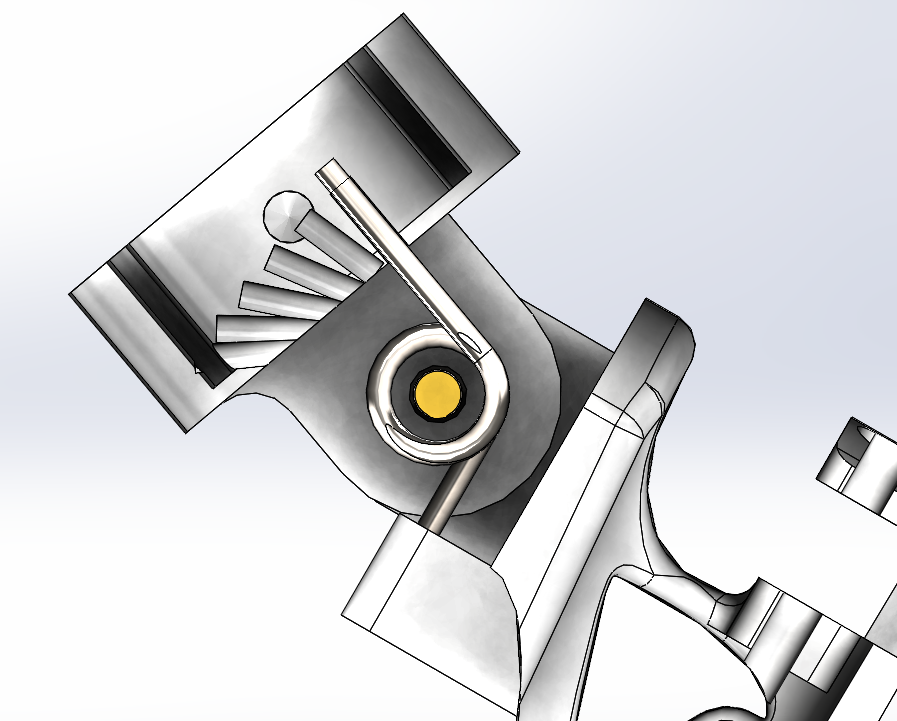
\includegraphics[width=0.75\textwidth]{figures/rotational_spring_rest_positions}
	\caption{Transversal section of the parallel spring resting positions in the left ankle.}
	\label{fig:rotational_spring_rest_position}
\end{figure}

\subsubsection{SEA + PEA configuration} % (fold)
\label{ssub:sea_pea_configuration}
The possibility of using both, SEA and PEA, configurations at the same time is given.
This lets the study of the combination of both configuration.
% subsubsection sea_pea_configuration (end)

\subsubsection{DD configuration } % (fold)
\label{ssub:dd_configuration}
Finally if no parallel spring is used and a spring stiff enough that doesn't add compliance to the system is placed, a DD configuration is achieved.
% subsubsection dd_configuration (end)

% subsection spring_integration (end)
%!TEX root = ../../../../report.tex

\subsection{Finite Element Method (FEM)} % (fold)
\label{sub:finite_element_method}
In sections \ref{sub:limb_profile} and \ref{ssub:rods}, a purely mathematical analysis has been carried out to calculate deformations and stresses on the limbs components.
This has been possible due to the simplification of the problem and the simple geometries utilized.
However, for more complex and critical parts a Finite Element Analysis (FEM) has been applied, in which the part is subdivided into small volumes and then analyzed individually.

As an example, in Figures \ref{fig:fem_foot_iteration_1} and \ref{fig:fem_foot_iteration_2}, an snapshot of the FEM in SolidWorks for the foot link can be seen.
The initial design of the sole was subject to this analysis and reinforced in the specially sensitive areas in order to meet a minimum deformation criteria.
However, all the mechanical designs tested here have always been also experimentally tried.
This is due to the fact that FEM studies are fully valid only under the condition of isomorphism for the materials which, in the case of 3D printed parts like the shown in the figures, is not true.
The FEM studies have been used more as a qualitative analysis rather than quantitative.

\begin{figure}[ht]
    \centering
    \begin{subfigure}[b]{0.49\textwidth}
        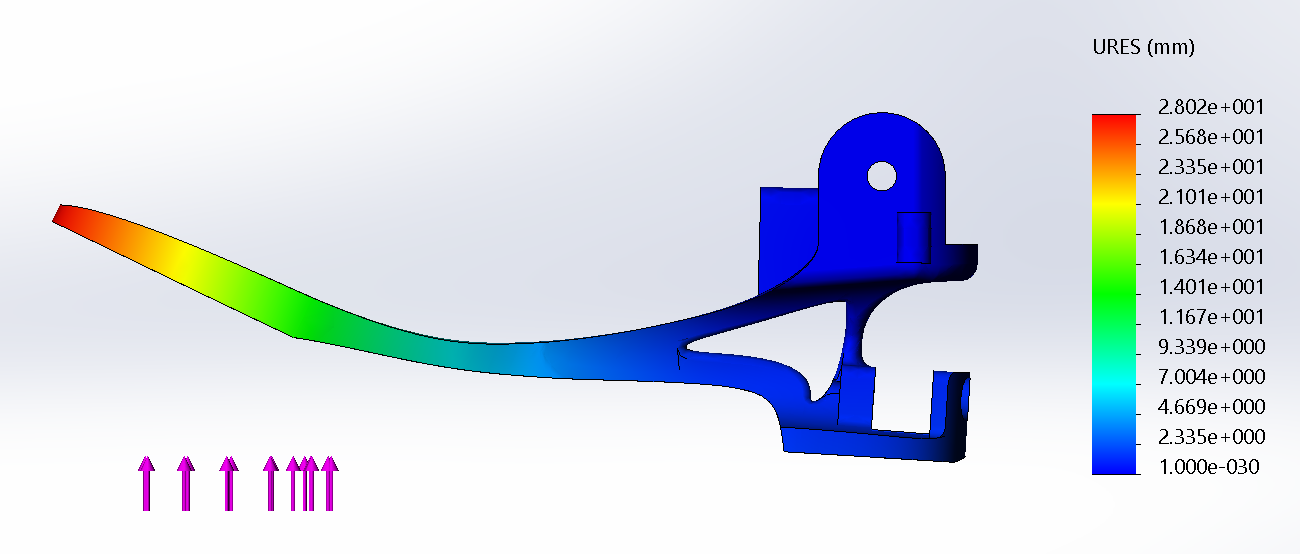
\includegraphics[width=\textwidth]{figures/fem_5N_1.PNG}
        \caption{FEM analysis in left foot iteration 1}
        \label{fig:fem_foot_iteration_1}
    \end{subfigure}
    \begin{subfigure}[b]{0.49\textwidth}
        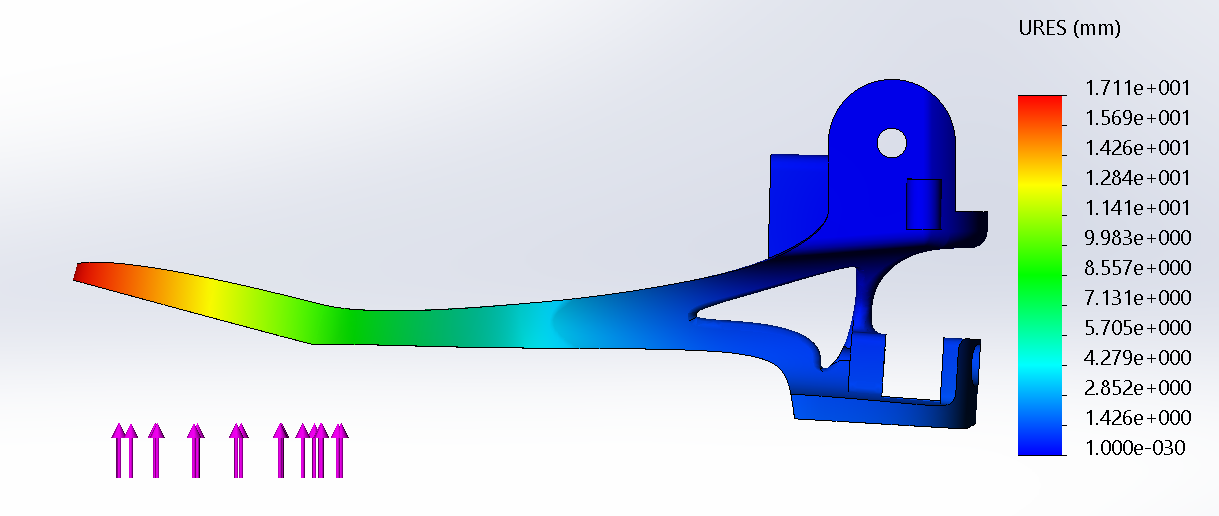
\includegraphics[width=\textwidth]{figures/fem_5N_2.PNG}
        \caption{FEM analysis in left foot iteration 2}
        \label{fig:fem_foot_iteration_2}
    \end{subfigure}
\end{figure}

% subsection finite_element_method (end)
%!TEX root = ../../../../report.tex
\subsection{Computer-Aided Design (CAD)} % (fold)
\label{sub:computer_aided_design}
After producing a final sketch for each component of the frame, the software SolidWorks was utilized to create their actual structure based on the required configuration, the desired placement of the sensors/actuators and wiring and the mechanical constraints calculated.
In the absence of precise data about the physical requirements of a component, its volume has been increased to reinforce the resistance of the piece.
When no mechanical or morphological constraints were to be applied, the criteria in CAD design has been mostly aesthetic, since the stile of the robot is worth considering, even if it does not influence its performance.

The CAD design has been carried out oriented to 3D-print manufacturing of the pieces, which adds new constraints in terms of resolution, size and materials available.
Some corrections had to be applied to the tolerances of the internal holes as explained in the section \ref{sub:arc_compensation} in order to avoid backslash.
However, the advantages of employing 3D printers for the construction of the prototype compensate for these limitations.

The implementation of the CAD design can be considered partially parametric due to the fact that a file with some parameters has been used in several parts.
This works so that in the reconstruction of the part, SolidWords reads the file and changes everything according to its content.
This has eased the iterative process of optimization of the manufactured components.
The values utilized are shown in the appendix \ref{app:cad_parameters}.
The results can be seen in the figures from \ref{fig:left_foot} to \ref{fig:knee_upper}.

\begin{figure}[ht!]
    \centering
    \begin{subfigure}[b]{0.49\textwidth}
        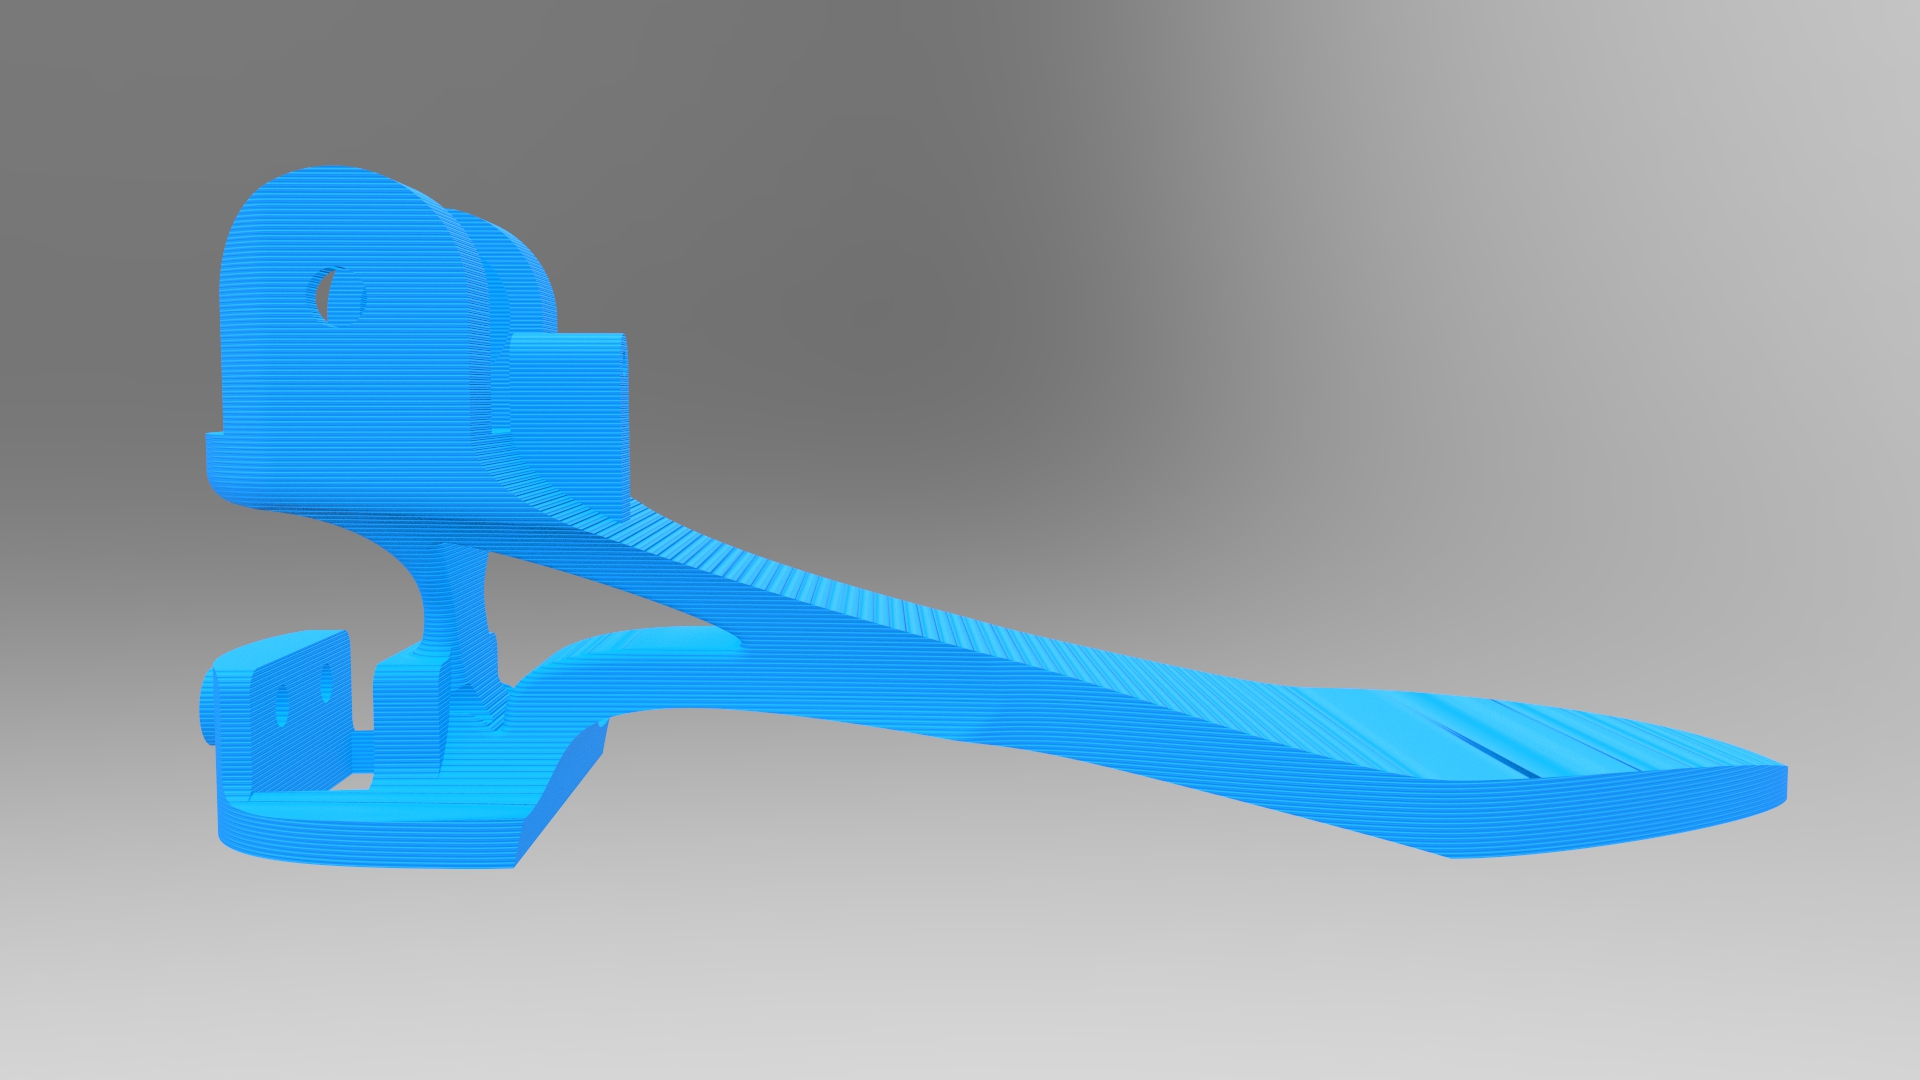
\includegraphics[width=\textwidth]{figures/legs_foot.jpg}
        \caption{Left foot}
        \label{fig:left_foot}
    \end{subfigure}
    \begin{subfigure}[b]{0.49\textwidth}
        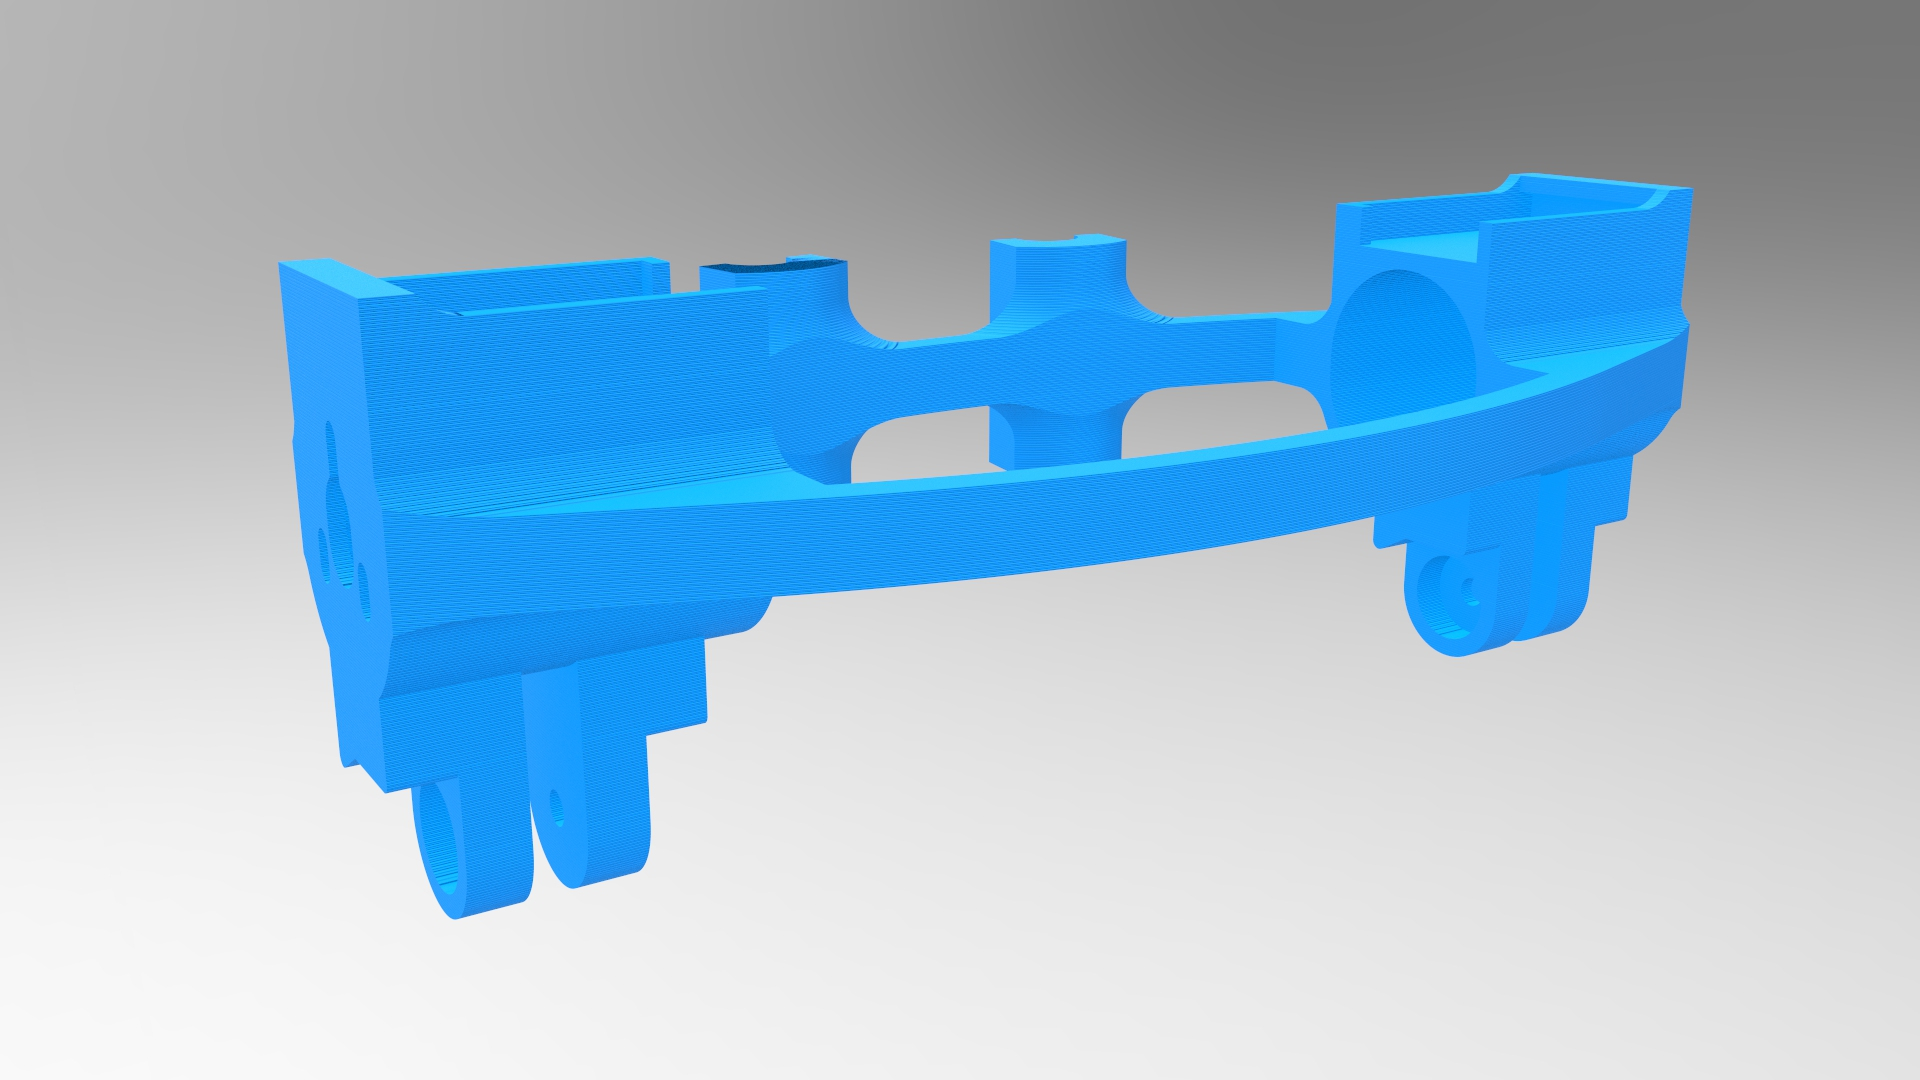
\includegraphics[width=\textwidth]{figures/legs_hip.jpg}
        \caption{Hip}
        \label{fig:hip}
    \end{subfigure}
\end{figure}    

\begin{figure}[ht!]
    \ContinuedFloat % continue from previous page
    \begin{subfigure}[b]{0.49\textwidth}
        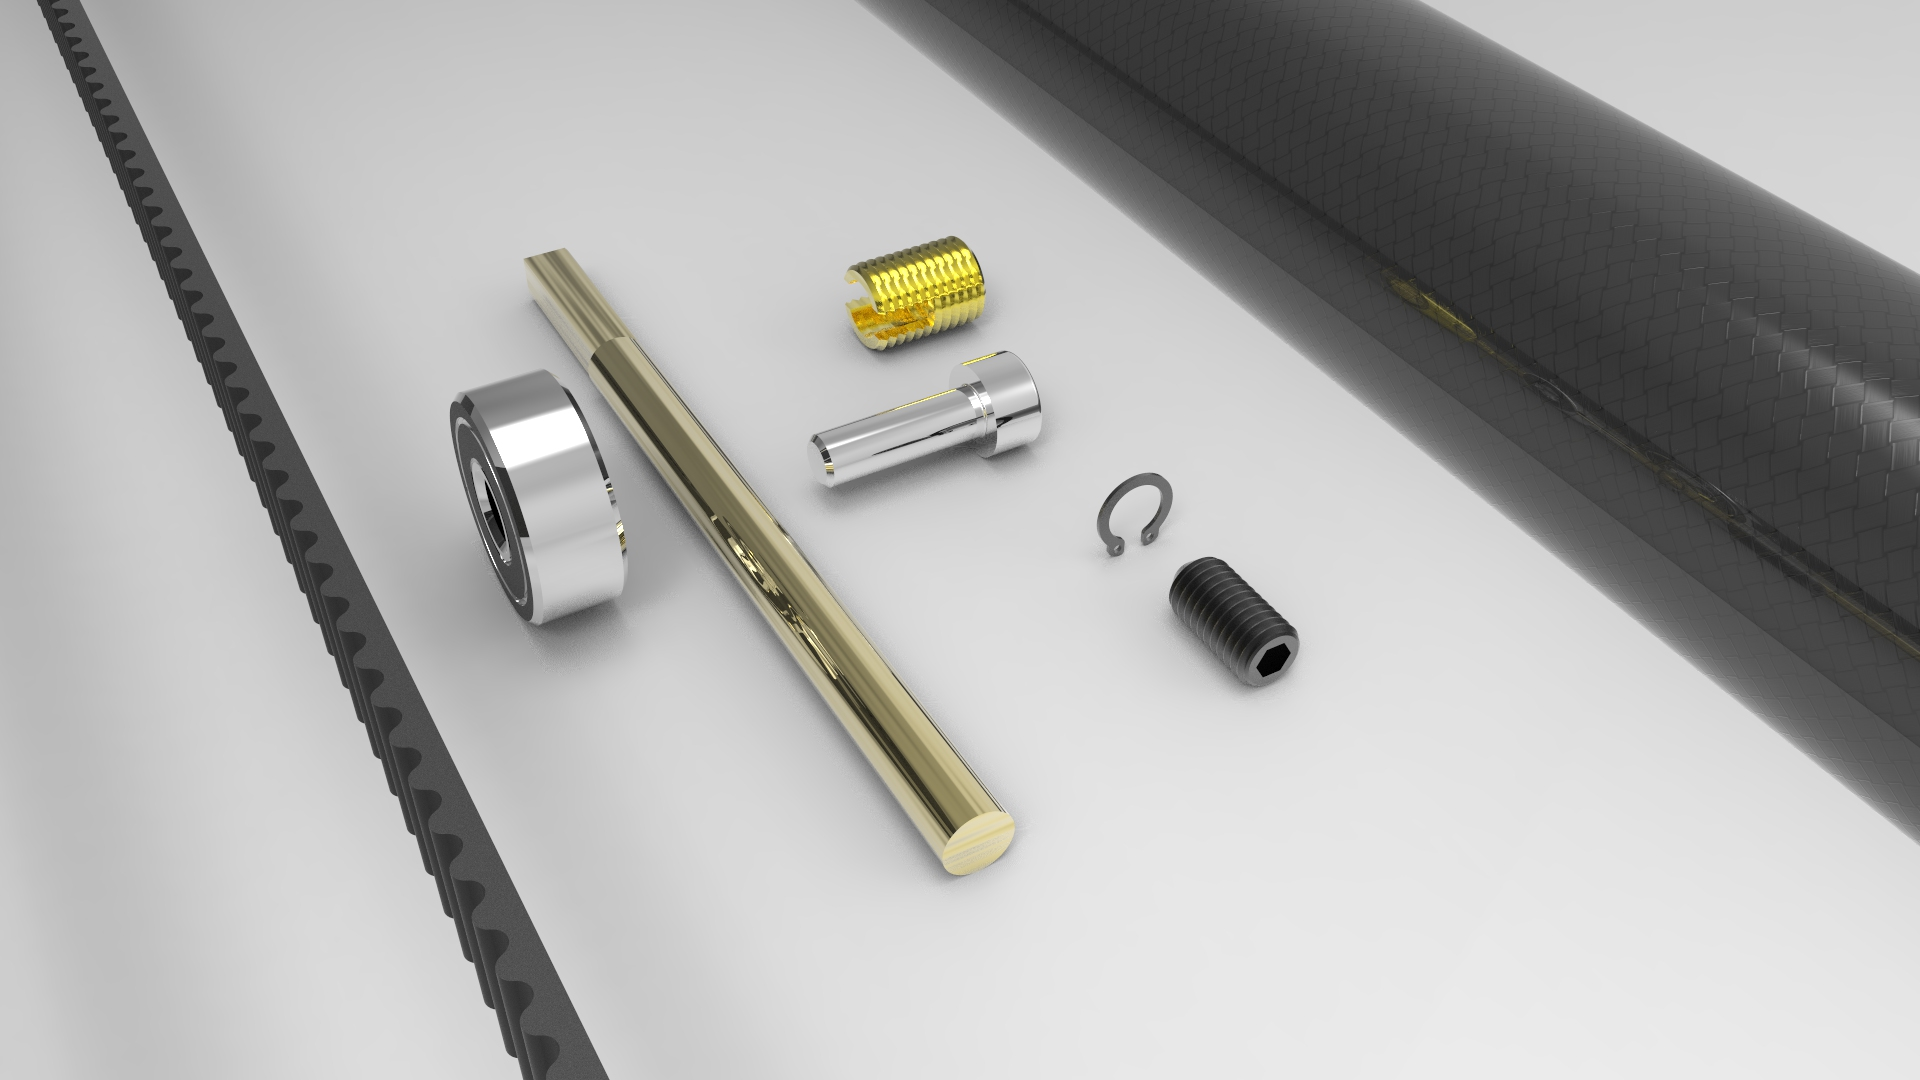
\includegraphics[width=\textwidth]{figures/legs_parts.jpg}
        \caption{Additional designed parts}
        \label{fig:mouse}
    \end{subfigure}
    \begin{subfigure}[b]{0.49\textwidth}
        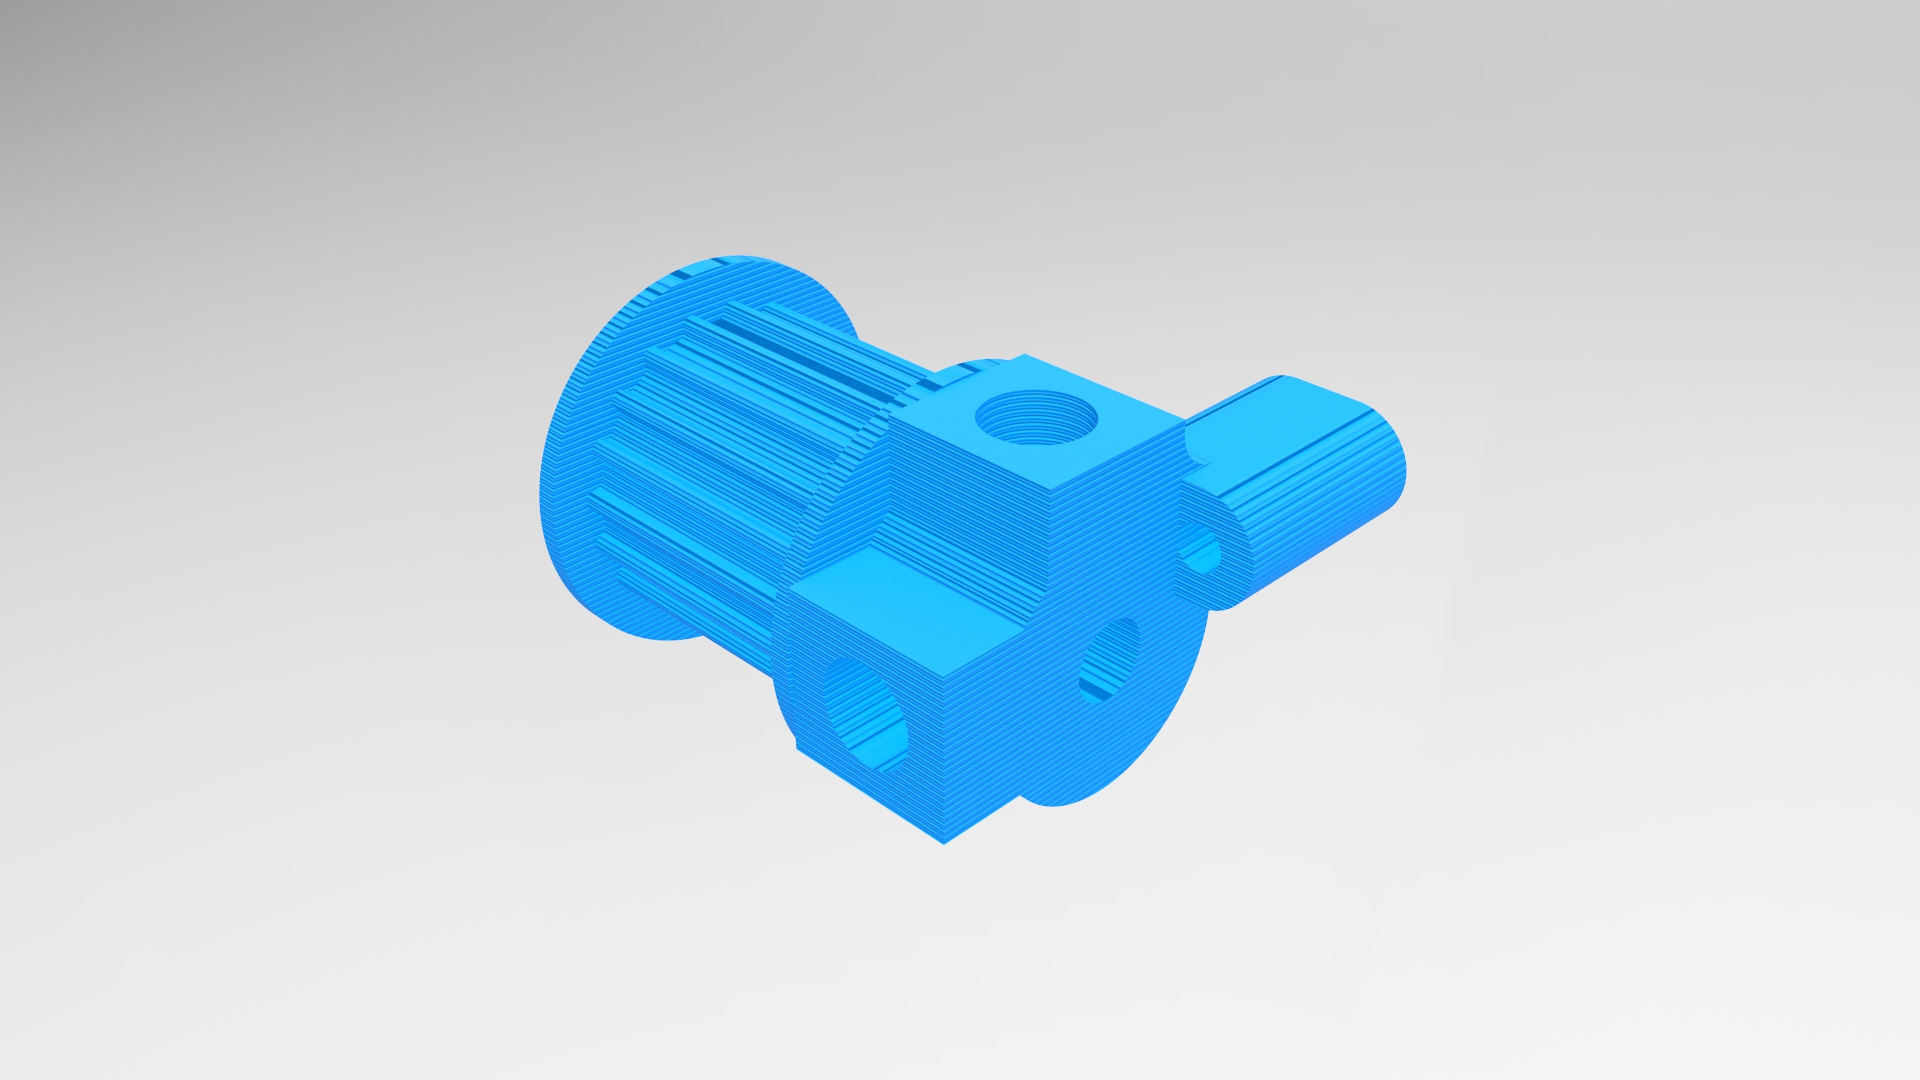
\includegraphics[width=\textwidth]{figures/legs_pulley.jpg}
        \caption{Left ankle serial spring pulley}
        \label{fig:serial_spring_pulley}
    \end{subfigure}
\end{figure}    

\begin{figure}[ht!]
    \ContinuedFloat % continue from previous page
    \begin{subfigure}[b]{0.49\textwidth}
        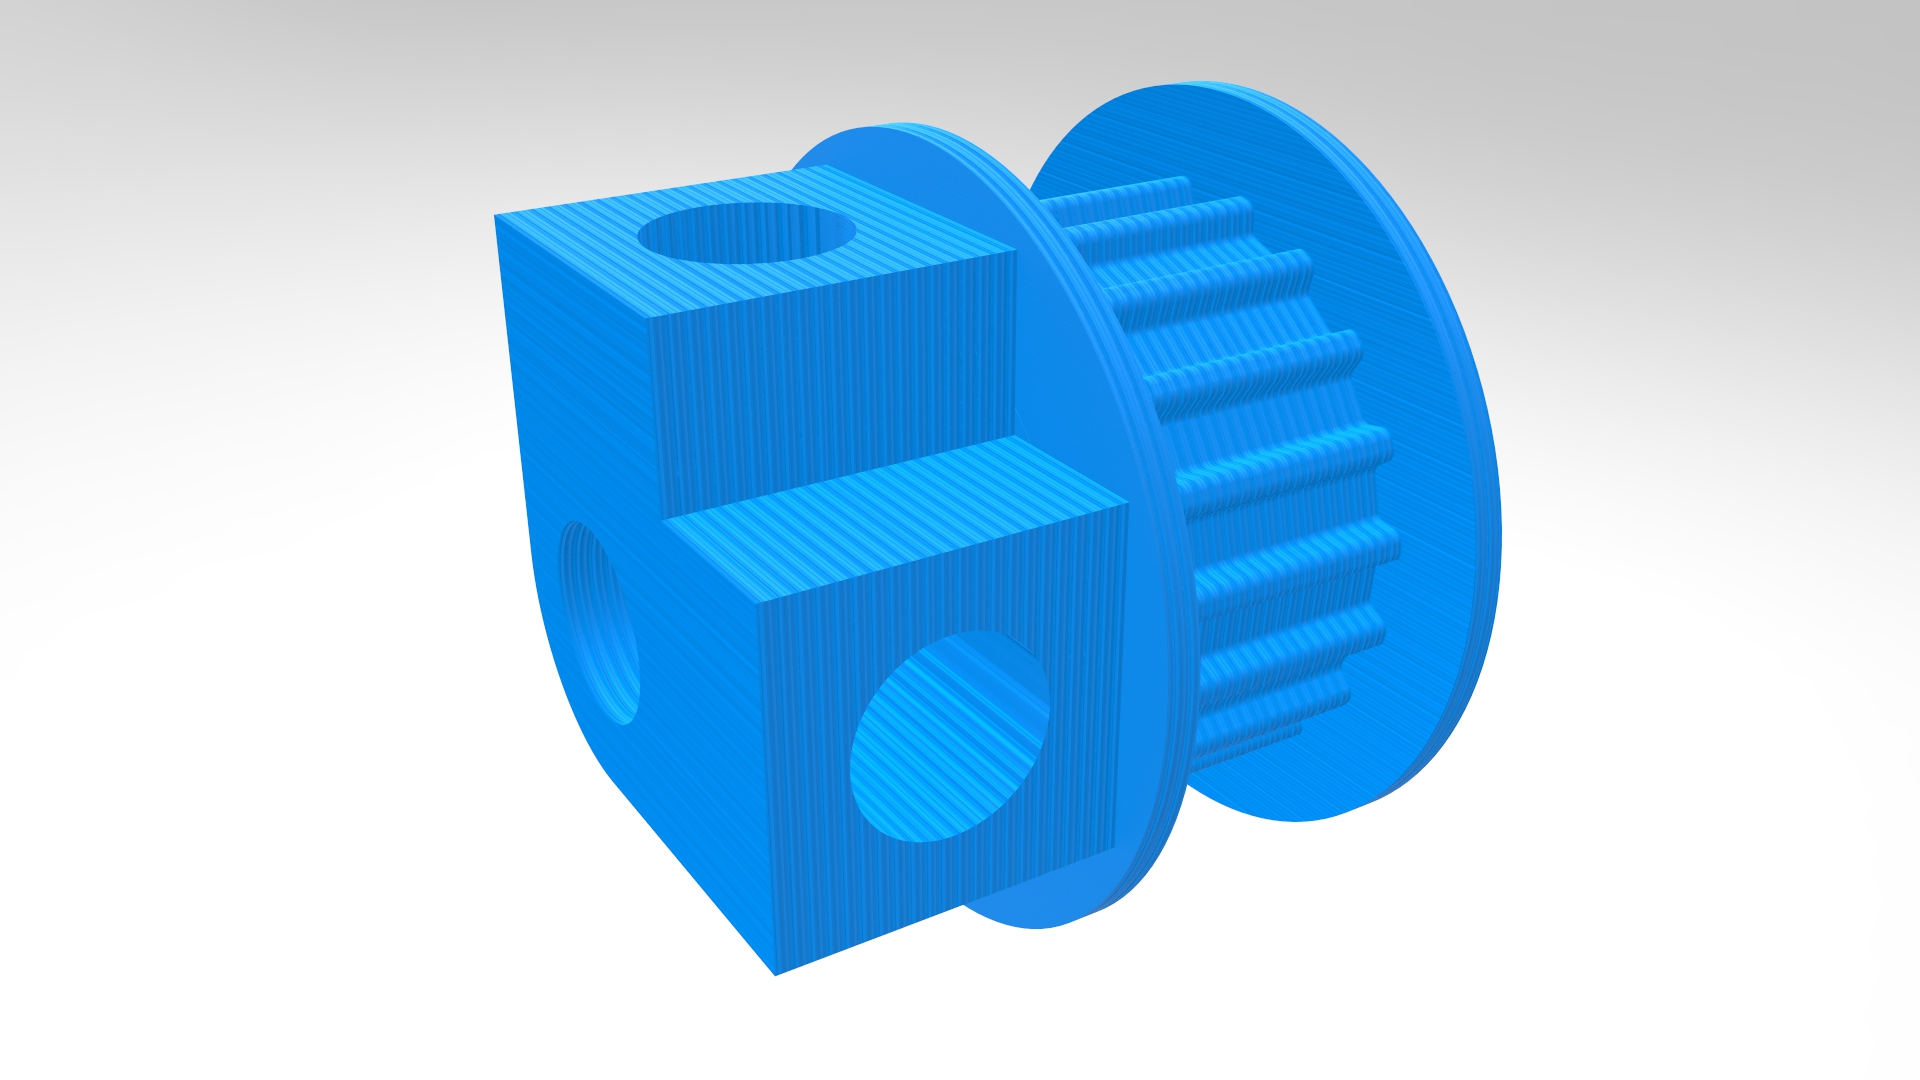
\includegraphics[width=\textwidth]{figures/legs_pulley_motor.jpg}
        \caption{Motor pulley}
        \label{fig:motor_pulley}
    \end{subfigure}
    \begin{subfigure}[b]{0.49\textwidth}
        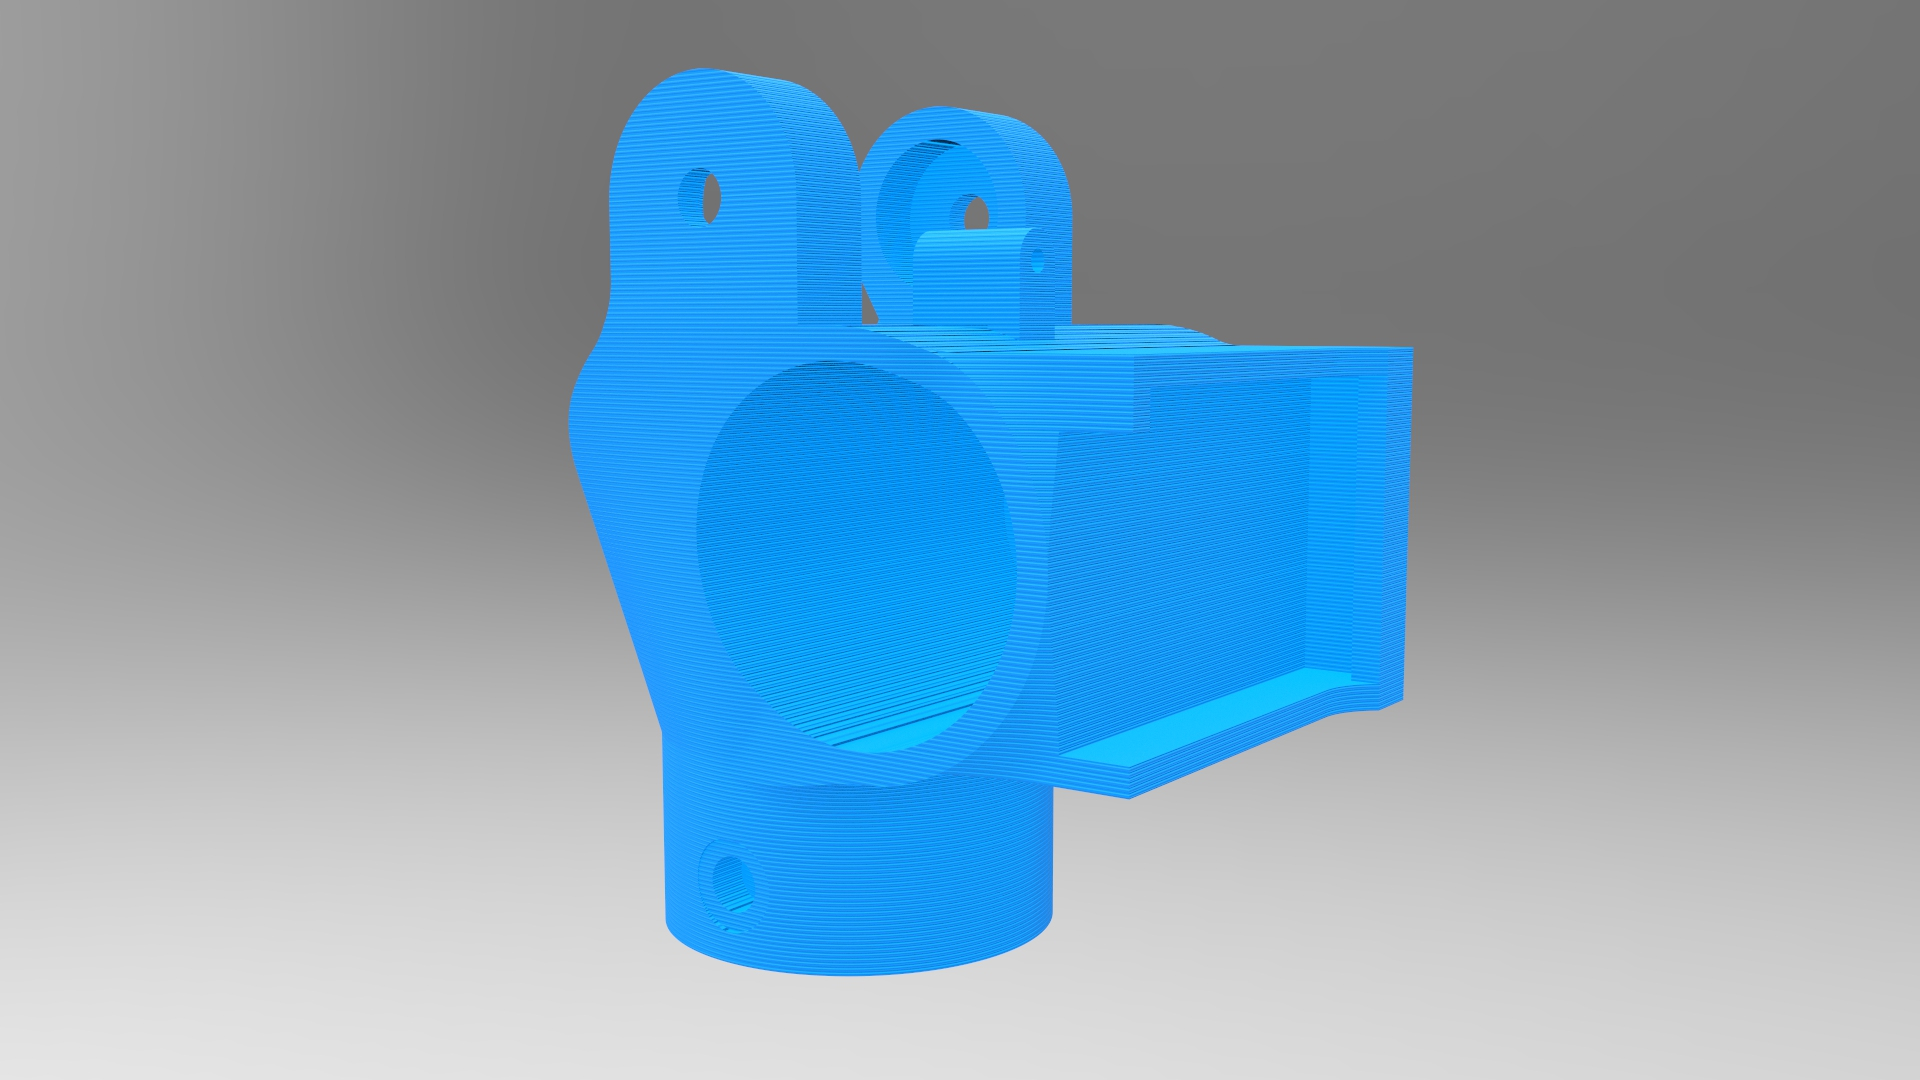
\includegraphics[width=\textwidth]{figures/legs_knee_lower.jpg}
        \caption{Left lower knee}
        \label{fig:lower_knee}
    \end{subfigure}
\end{figure}

\begin{figure}[ht!]
    \ContinuedFloat % continue from previous page
    \begin{subfigure}[b]{0.49\textwidth}
        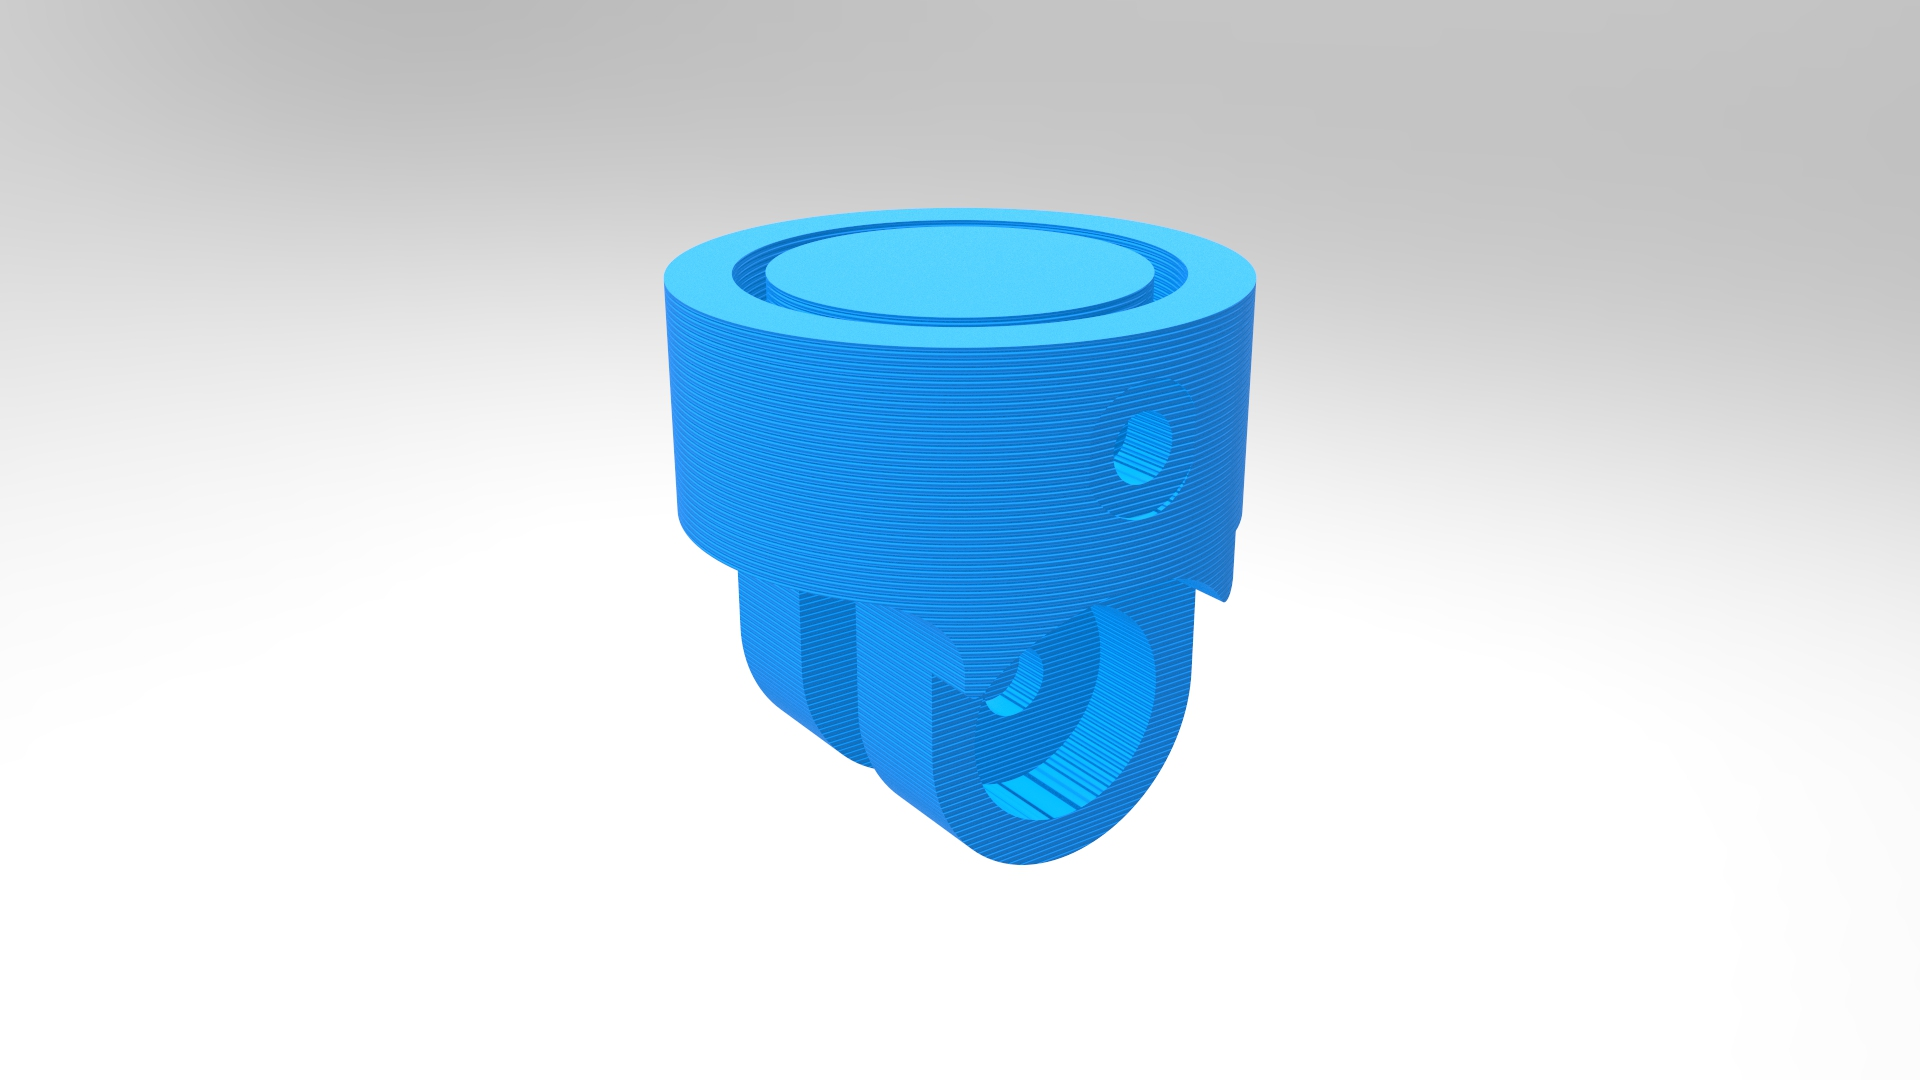
\includegraphics[width=\textwidth]{figures/legs_ankle_upper.jpg}
        \caption{Left upper ankle}
        \label{fig:ankle_upper}
    \end{subfigure}
    \begin{subfigure}[b]{0.49\textwidth}
        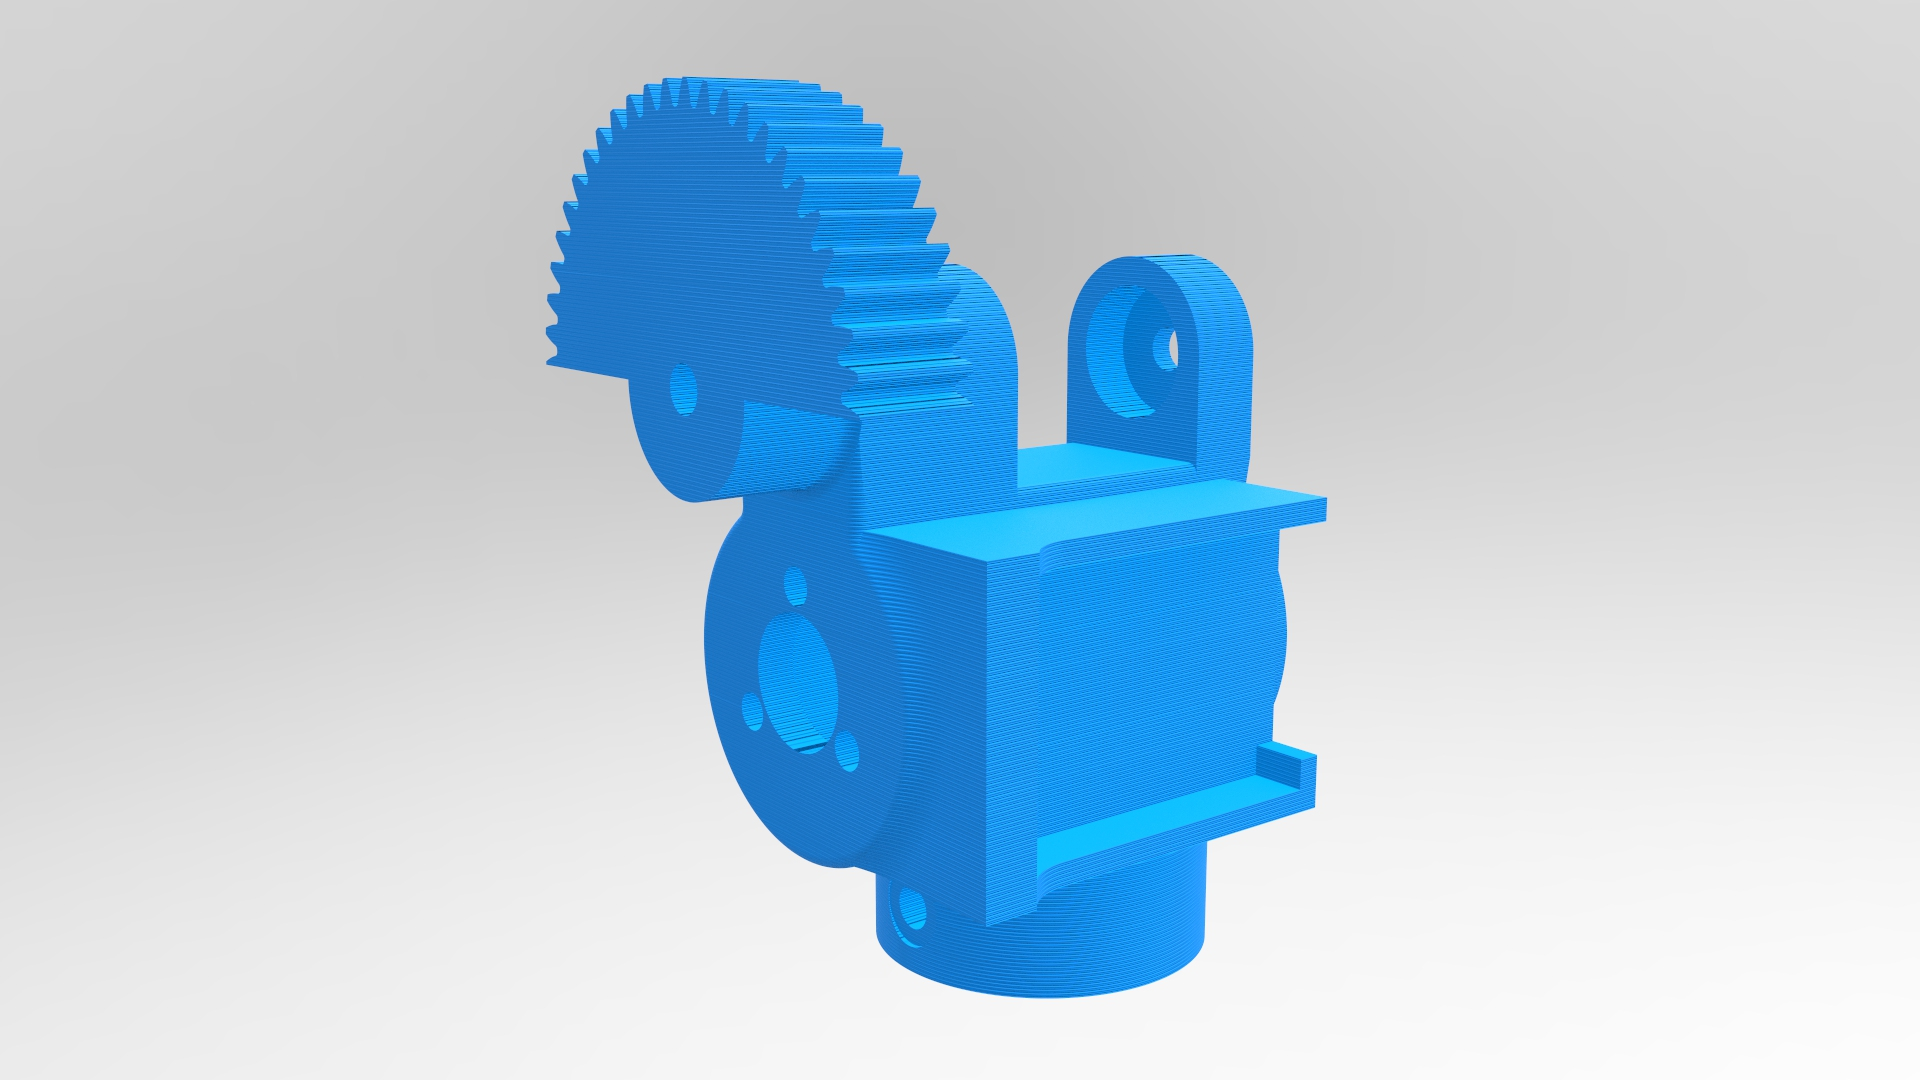
\includegraphics[width=\textwidth]{figures/legs_hip_lower.jpg}
        \caption{Left lower hip}
        \label{fig:hip_lower}
    \end{subfigure}
\end{figure}

\begin{figure}[ht!]
    \ContinuedFloat % continue from previous page
    \begin{subfigure}[b]{0.49\textwidth}
        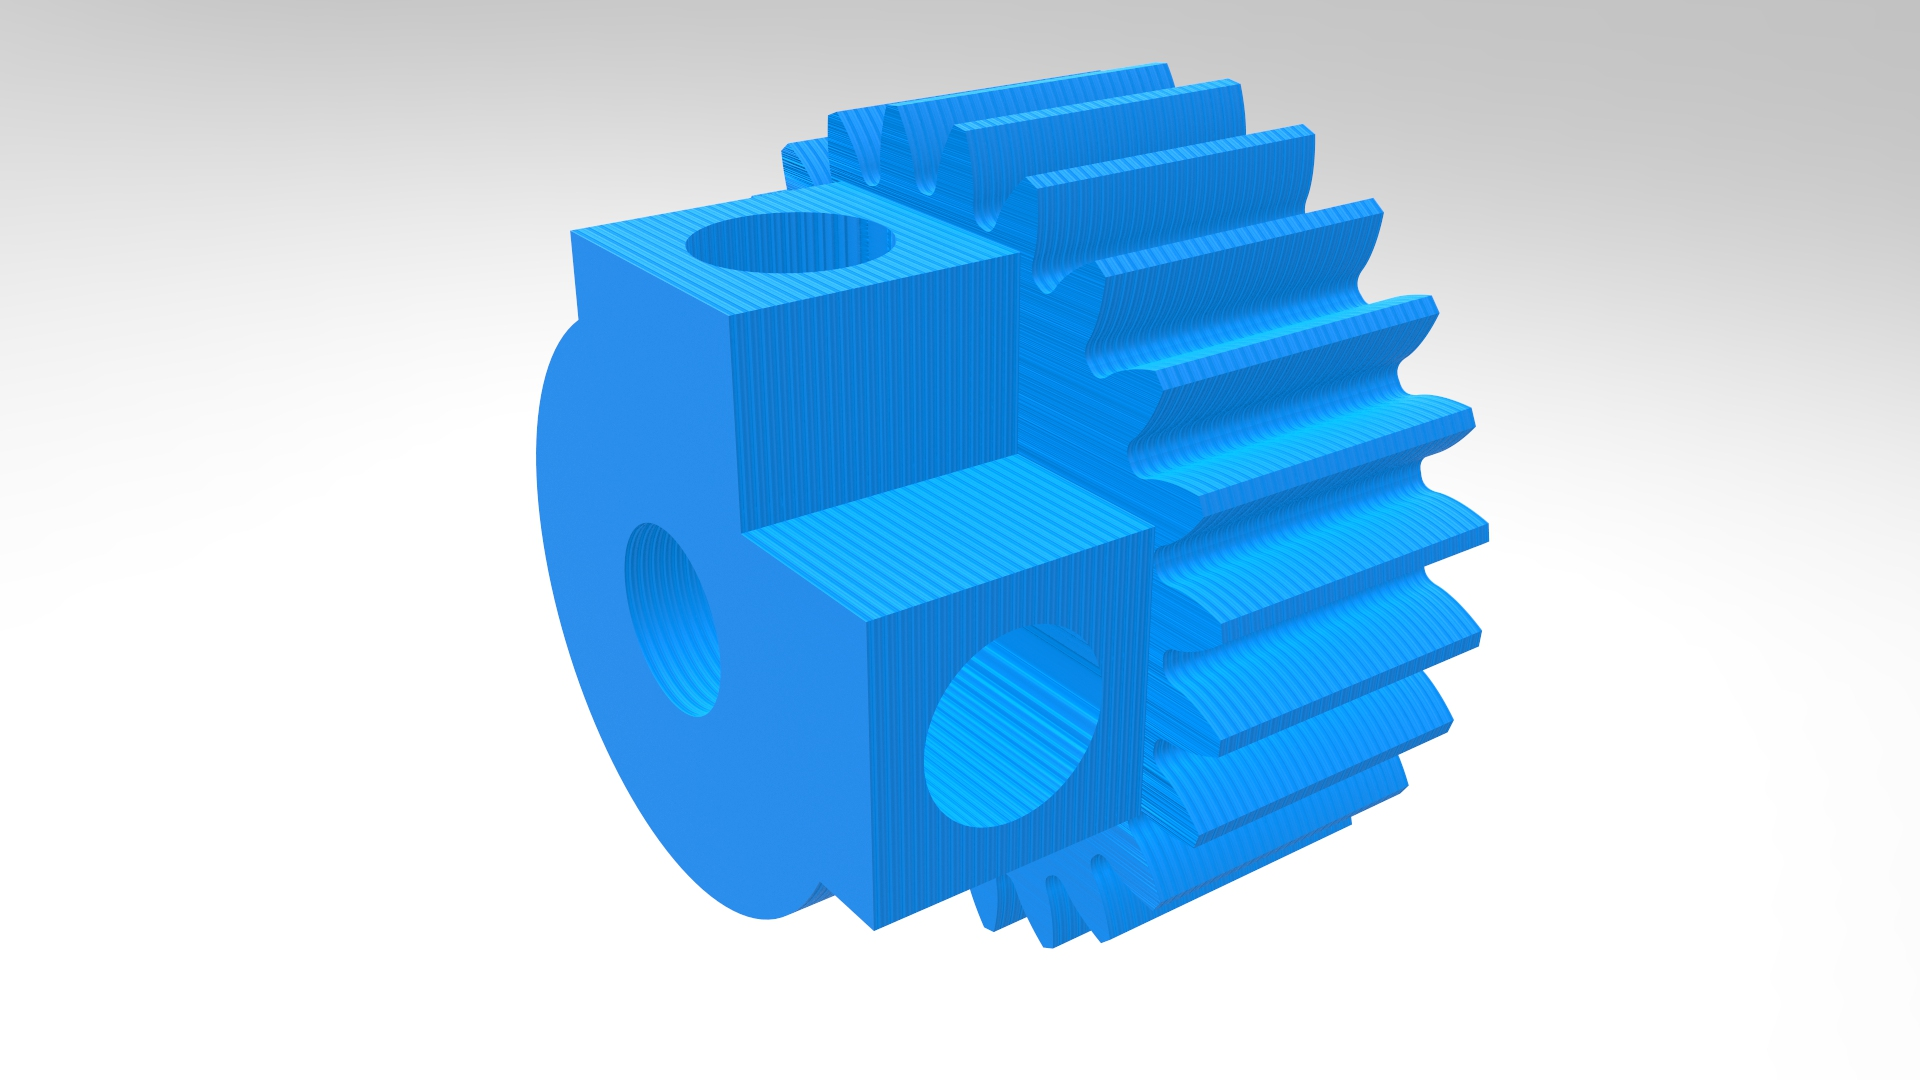
\includegraphics[width=\textwidth]{figures/legs_hip_pinion.jpg}
        \caption{Hip's pinion}
        \label{fig:hip_pinion}
    \end{subfigure}
    \begin{subfigure}[b]{0.49\textwidth}
        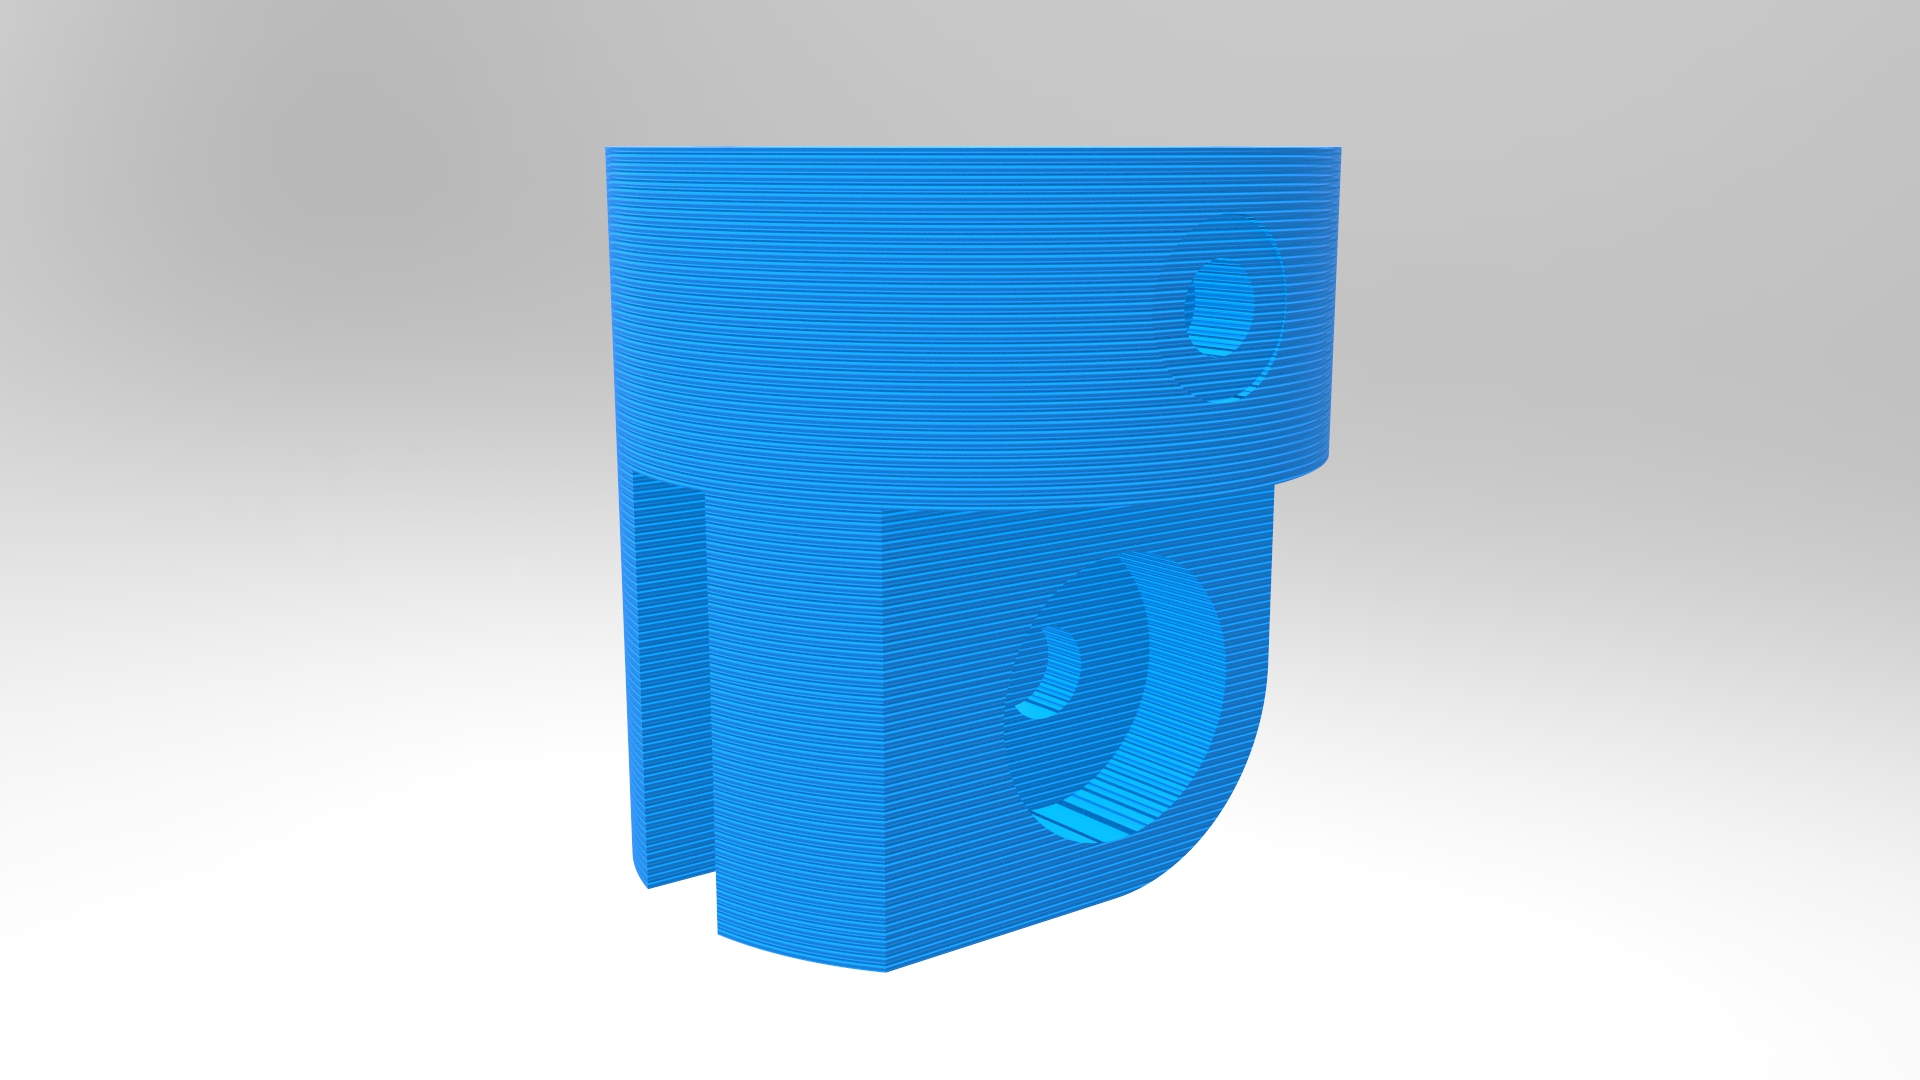
\includegraphics[width=\textwidth]{figures/legs_knee_upper.jpg}
        \caption{Left upper knee}
        \label{fig:knee_upper}
    \end{subfigure}
    \caption{Main CAD designed components}
\end{figure}

The CAD program has the feature of, given the physical properties of the materials used, calculate the geometrical values of a component such as moments of inertia or CoM position.
This has been used in the construction and use of the mathematical model in \ref{cha:mathematical_model} and to size the motors, or in the simulation \ref{cha:simulation} to create the model as close to reality as possible.
The table \ref{tab:limb_physical_properties} contain the moments of inertia and total mass calculated by the CAD program.
The moments of inertia are taken from the appropriate rotation axis of the link.

% subsection computer_aided_design (end)
%!TEX root = ../../../../report.tex
\subsection{Mechanical limits of the joints} % (fold)
\label{sub:mechanical_limits}
The implementation of mechanical limits for the joints obeys to two reasons:
\begin{enumerate}
  \item \textbf{Calibration}: they can be used as starting, known positions for the relative encoders.
  \item \textbf{Security}: a mechanical limit will restrict the movements and prevent any configuration non-natural or dangerous for the physical integrity of the robot.
\end{enumerate}

The Figure \ref{fig:joint_limits_hip} depicts how the mechanical limits of the hip (both left and right) are implemented in the upper part, comprising an angle of 90 + 60 = 150 degrees.
Figure \ref{fig:joint_limits_ankle_upper} shows the upper part of the ankle and how the allowed movement of the foot has a range of 60 + 50 = 110 degrees.
The mechanical limits of the knee are obtained as a combination of the lower and upper components of the joint.
These allow movements of 0 + 120 = 120 degrees as shown in the figures \ref{fig:joint_limits_knee_upper} and \ref{fig:joint_limits_knee_lower}.
The angles of the mechanical limits have been calculated according to the physical limitations in humans.

\begin{figure}[ht!]
    \centering
    \begin{subfigure}[b]{0.49\textwidth}
        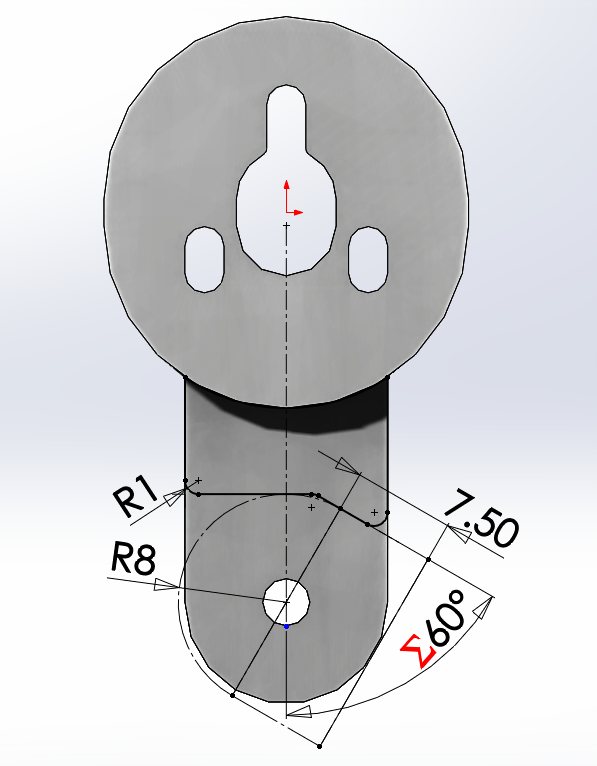
\includegraphics[width=\textwidth]{figures/joint_limits_hip.PNG}
        \caption{Joint limits of the hip}
        \label{fig:joint_limits_hip}
    \end{subfigure}
    \begin{subfigure}[b]{0.49\textwidth}
        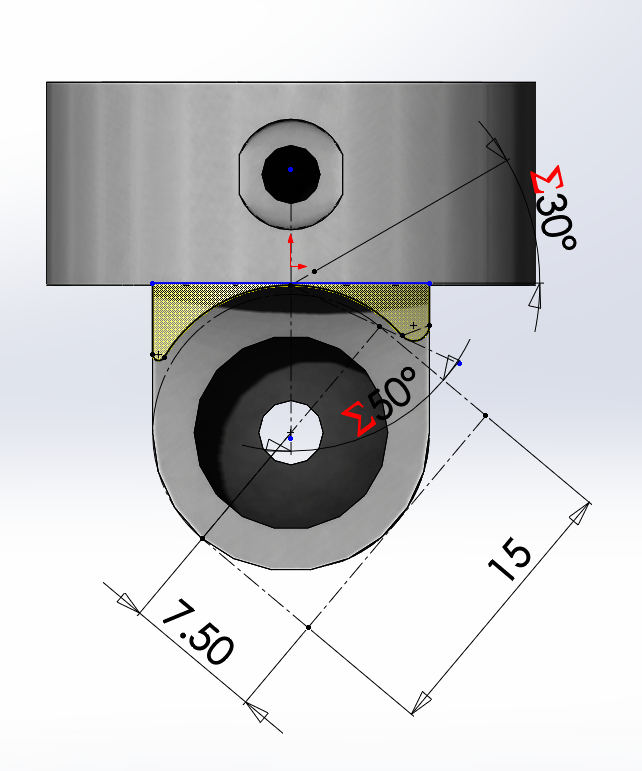
\includegraphics[width=\textwidth]{figures/joint_limits_ankle_upper.PNG}
        \caption{Joint limits of the ankle}
        \label{fig:joint_limits_ankle_upper}
    \end{subfigure}
\end{figure}    

\begin{figure}[ht!]
    \ContinuedFloat % continue from previous page
    \begin{subfigure}[b]{0.49\textwidth}
        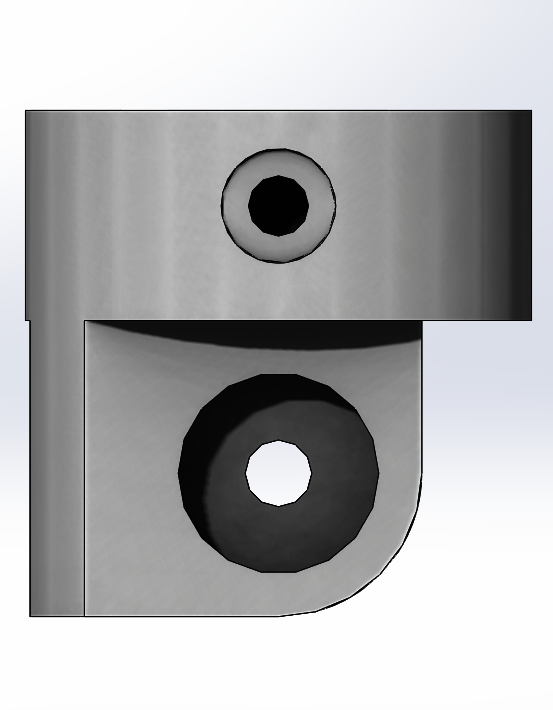
\includegraphics[width=\textwidth]{figures/joint_limits_knee_upper.PNG}
        \caption{Joint limits of the knee: Upper link}
        \label{fig:joint_limits_knee_upper}
    \end{subfigure}
    \begin{subfigure}[b]{0.49\textwidth}
        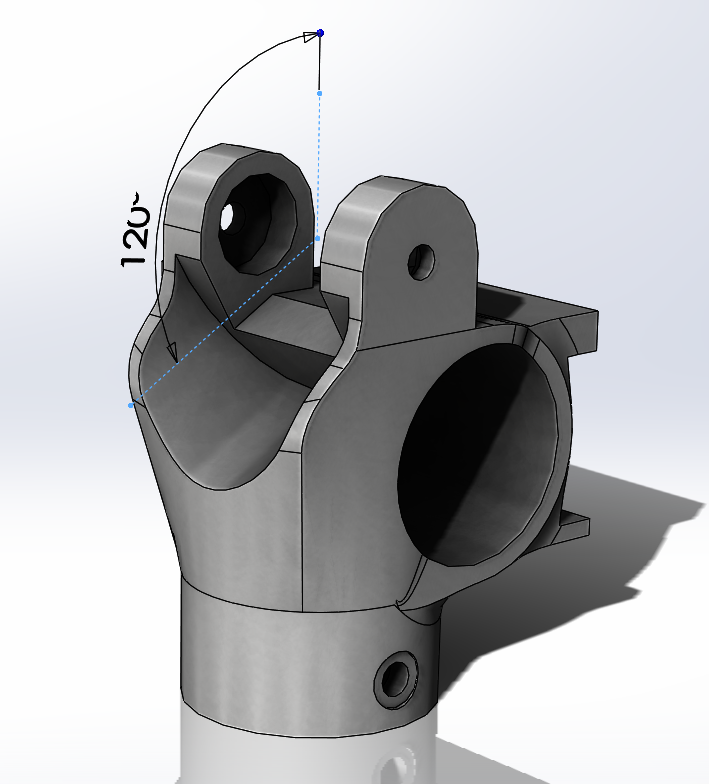
\includegraphics[width=\textwidth]{figures/joint_limits_knee_lower.PNG}
        \caption{Joint limits of the knee: Lower link}
        \label{fig:joint_limits_knee_lower}
    \end{subfigure}
\end{figure}    

% subsection mechanical_limits (end)

% section mechanics (end)
%!TEX root = ../../../report.tex
\vfill
\section{Software} % (fold)
\label{sec:software}

%!TEX root = ../../../../report.tex

\subsection{Motivation} % (fold)
\label{sub:motivation}
When approaching the task of designing a new robotic platform for the AI department at the Mærsk Mc-Kinney Møller Institute, the current development environment being utilized and its capabilities were studied as a first step.
Nowadays, the simulation and control of the robots at the department is based on the LPZrobots \cite{lpzrobots} and Gorobots \cite{gorobots} packages.
These software tools provide both a simulation engine for robots built on ODE \cite{ode}, OSG \cite{osg} and a framework for an easy implementation of controllers in both simulation and hardware.
However, their specificity compared to other existing instruments collides with some of the core design ideas of the robot framework presented here, which are simplicity of use and generalization.
The above mentioned are the reasons why it was decided to migrate the development environment to ROS Jade \cite{ros} for the bipedal locomotion study framework of RuBy. 

% subsection motivation (end)
%!TEX root = ../../../../report.tex

\subsection{ROS Control} % (fold)
\label{sub:ros_control}
Within the Robot Operating System libraries, the ROS Control set of packages \cite{ros_control} contains several tools specially conceived for a generalized a simple implementation of robot controllers.
Besides, it standardizes the use of Gazebo \cite{gazebo} as a simulation environment with ROS by providing the necessary interfaces in conjunction with a simple plugin\footnote{The implementation of the simulation environment for RuBi in Gazebo and its adaption to ROS are discussed in \ref{cha:simulation}.}.
The architecture of the simulation, hardware, controllers and transmissions modules created through ROS control for both the Gazebo simulation environment and the a robot can be seen in Figure \ref{fig:ros_control_gazebo}, as from the tutorial in \cite{ros_control_tutorial}. The reader is referred to this online tutorial for a detailed explanation of the general features and the setup instructions of all the necessary modules discussed in this section.

\begin{figure}[ht]
	\centering
	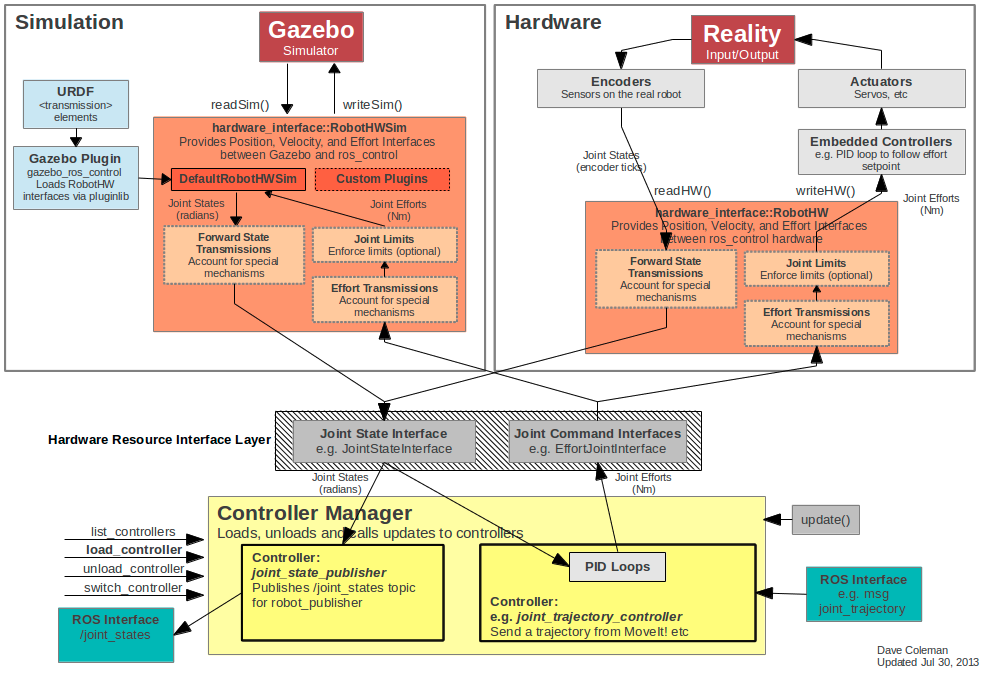
\includegraphics[width=\textwidth]{figures/ros_control_gazebo.png} 
	%Se que no te gusta, gordo, pero no la he encontrado en mejor calidad y son las 6 am
	\caption{ROS Control and Gazebo data flow.}
	\label{fig:ros_control_gazebo}
\end{figure}

This architecture is meant to handle in real-time all the intermediary steps between the generation of joint commands for the robot by the custom controllers and their use in the platform, as well as for the feedback information flow in the opposite direction.
The idea behind it is that for most of the actuator and sensor types in a robot joint, the basic commands and readings can be abstracted to a few kinds, being currently implemented position, velocity and effort instances.
ROS control offers a set of controllers and transmissions for dealing with their transfer through the Hardware Resource Interface Layer, the Control Manager and the Controller modules in Figure \ref{fig:ros_control_gazebo}.
That leaves the "hardware interface" modules as the only part that needs to be defined by the user since they are platform dependent.
The interface with the real robot is discussed in \ref{sub:ros_control_hardware_locokit_interface}, while the one with the simulation is introduced in \ref{cha:simulation}.


% subsection ros_control (end)
%!TEX root = ../../../../report.tex
\subsection{ROS Control-to-Hardware interface} % (fold)
\label{sub:ros_control_hardware_locokit_interface}
The Locokit embedded electronics comes along a standard C library called LocoAPI designed for an easy interaction and use of the capabilities of its hardware, as presented in \cite{locokit}.
This library has been utilized to implement the basic hardware functionalities in RuBi without any modification.
However, it can be easily edited or extended in order to add new ones if needed, which was considered a great advantage during the selection of the hardware platform.

The Locokit can be configured to offer a wireless interface between its main processor and an external computer creating and add-hoc WiFi network in the Gumstix.
Besides, it offers a ready-to-use $C$ application based on the LocoAPI to work as the server side when interfacing the hardware. \ref{} \todo{add actuateMotors.c to code stack?}
Its setup and use instructions can be found in the Locokit documentation, supplied with the kit.
This left the client side of the wireless connection as the one that needed to be created.
An existing client application built as an "AbstractController" for the LPZrobots framework was already available. 
However, as explained before, to eliminate any dependency with LPZrobots and in order to use it within ROS Control, it was rewritten as an instantiation of "RobotHW" making use of the LocoKitInterface and ConnectionClass $C++$ classes provided.

\subsubsection{The Locokit HW interface node} % (fold)
\label{ssub:the_locokit_hw_interface}
The resulting ROS node currently implements the functions listed in \ref{list:locoHW_functions}.
They are fully operative and have been tested before assembling the actuators to the joints.

\begin{itemize}
\label{list:locoHW_functions}
	\item Setup of wireless connection: connect to the TCP websocket created in the server side. It requires the IP and port on the server side.
	\item Registration of HW interface handlers for ROS Controller Manager: currently Effort commands and Joint State readings can be transmitted.
	\item Transmission of motor commands to motor boards in HW side: PWM signal values. It requires the physical addresses of all the motor boards connected.
	\item Reception of joint state readings from motor boards: encoder tics for relative position.
	\item Real-time handling of information transfer from/to the Controller Manager.
\end{itemize}

The node can be extended with new standard/customized HW interface handlers and more functions from the "LocokitInterface" class for future applications.
However, it lacks some capabilities that will be of relevance for an optimal functioning of the RuBi robot and that failed be implemented due to time constraints or lack of resources. 
The main ones are listed in \ref{list:locoHW_functions_left}.

\begin{itemize}
\label{list:locoHW_functions_left}
	\item An initialization of the encoders to a predefined position set as zero in order to compute absolute position values.
	\item A new data flow channel to manage the sensory feedback information from non-built-in sensors, at the ground contact switches.
	\item If necessary, a mapping between the Effort command values received from the controller and the valid PWM signals sent to the motors.  
\end{itemize}
% subsubsection the_locokit_hw_interface (end)

% subsection ros_control_hardware_locokit_interface (end)
%!TEX root = ../../../../report.tex

\subsection{Custom controllers} % (fold)
\label{sub:example_controllers}
From the \textit{Controller manager} in ROS Control, a variety of joint handlers are offered.
Among them, in the created controllers \textit{Impulse controller} and \textit{Two-neuron controller} the position and effort handlers are used individually for each joint.
Thus, these controllers provide a ROS topic (e.g. /rubi/left\_ankle\_position) that the user can employ to move the actuators or read from the sensors.
The joint handlers are created from a unique package called \textit{rubi\_joint\_controllers}.
It is worth mentioning here that the position handlers used for the joints contain a PID whose values have been adjusted experimentally through the simulations for each joint.

Two type of controllers are given that show a different range of options to use with the robot.
Both are gathered in a sole package called \textit{rubi\_controllers}, which gives a more organized and resource-shared environment rather than having a package for each controller.
This also eases the creation of packages for new custom controllers by providing an example package.
In order to start a new piece of code this must be created and then added in the \textit{CMakeLists.txt} from where also some examples are included.
The presented code follows the ROS conventions and the code style is the \textit{Google style} offered by the clang-code-model.
This creates a congruent workspace monitored by a git repository.

\subsubsection{Two-neuron controller} % (fold)
\label{ssub:two_neuron_controller}
This first example controller shows how to:
\begin{enumerate}
    \item Use GoRobots.
    \item Make use of dynamic reconfigure.
    \item Adapts its behavior depending on Gazebo the real time factor.
\end{enumerate}
For the first, an example of how to link C++ code from GoRobots is shown in the \textit{CMakeLists.txt}.
This system is easier and more powerful than the current \textit{Makefiles} currently used in GoRobots.
The Artificial Neuronal Network (ANN) library is used to create a bi-neuronal network that creates the CPG signals of the actuators.
Furthermore, the synaptic weights can be modified by making use of the ROS feature \textit{Dynamic Reconfigurable Parameters}.
These offer an interface in order to change, on the fly, the the values of the created parameters.
In the Figure \ref{fig:rqt_interface}, an RQT workspace containing the CPG signals and the dynamic reconfigurable parameters modifiers is depicted.

\begin{figure}[tb]
    \centering
    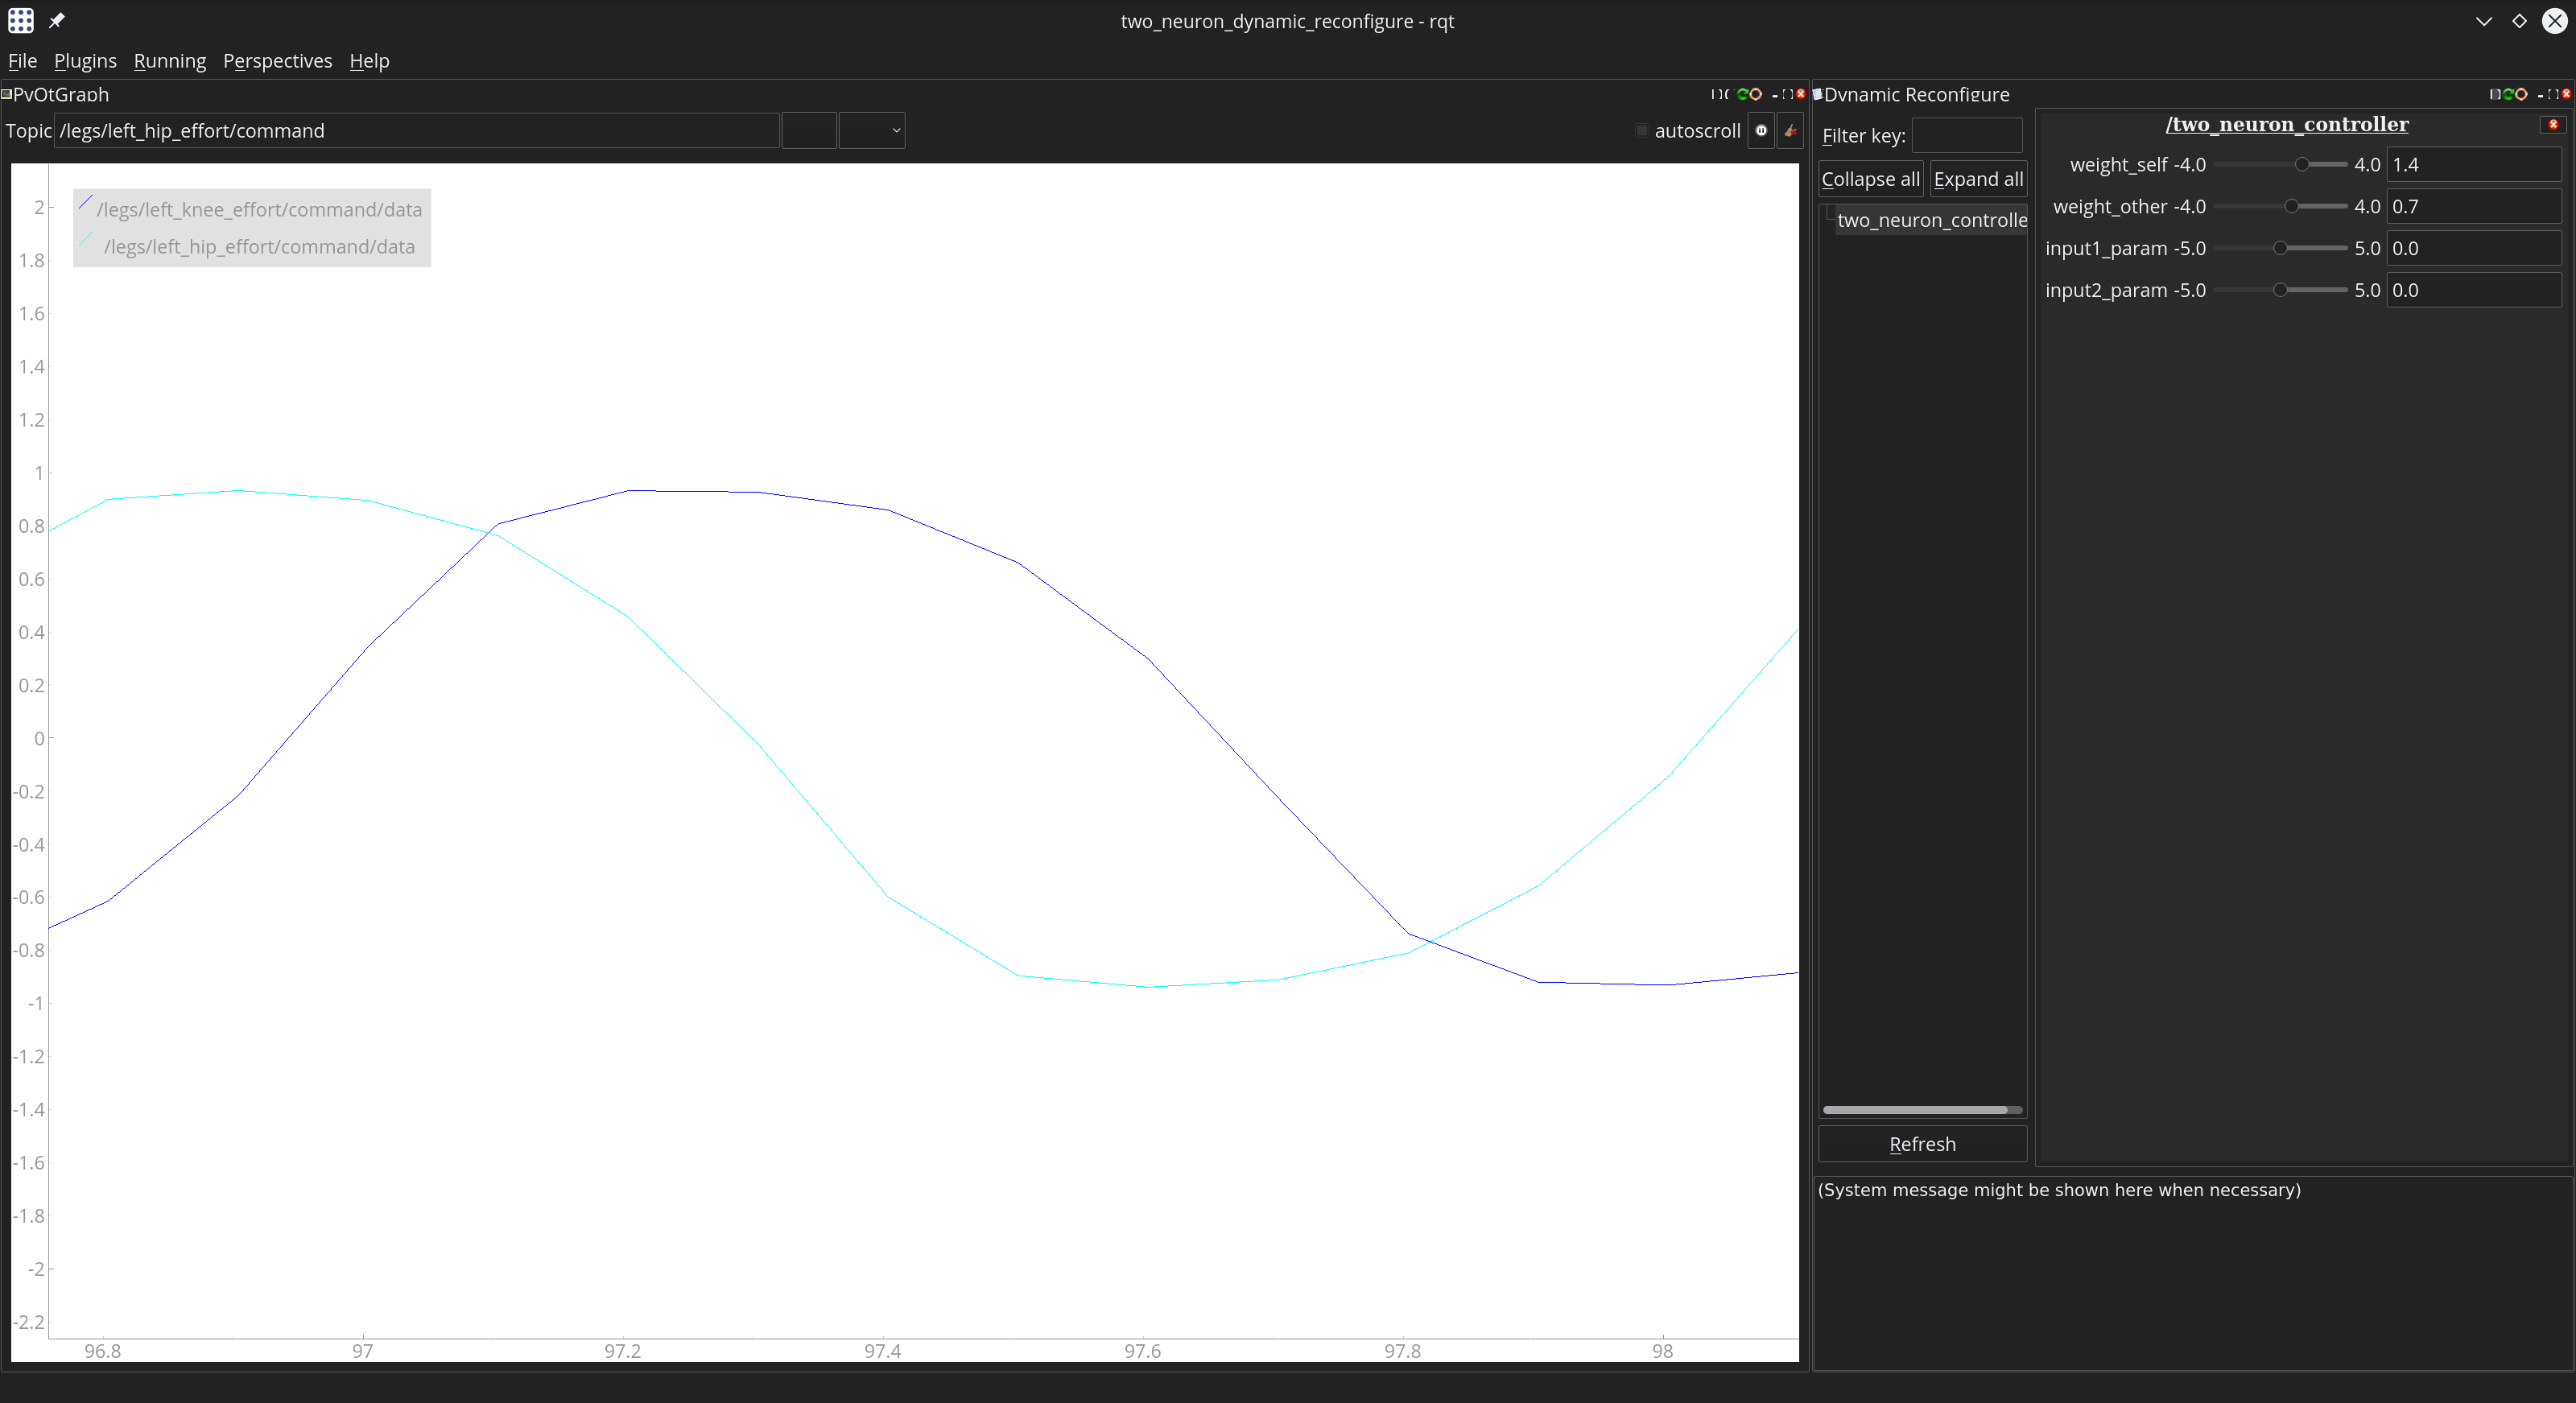
\includegraphics[width=\textwidth]{figures/rqt_interface}
    \caption{RQT workspace containing the CPG signals and the dynamic recofigurable parameters.}
    \label{fig:rqt_interface}
\end{figure}

These are also used to change the behavior of the ANN in order to be adapted to changes in Gazebo.
Gazebo users can modify the relationship between the simulation and computation times.
This is adjusted with a \textit{real time factor} that is read by the node and used to adjust the frequencies of the CPGs.
% subsubsection two_neuron_controller (end)

\subsubsection{Impulse controller} % (fold)
\label{ssub:impulse_controller}
Among other things this node shows how to:
\begin{enumerate}
    \item Load and unload different joint controllers.
    \item Give some wrappings for set of controllers (hoping position).
    \item Offer services for jumping: given a file or given the values and impulse time.
\end{enumerate}
This node implements some methods that enable it to change on-the-fly the handlers of each individual joint.
Furthermore, three combinations of individual joint handlers are given, being these: (1) all in position mode, (2) all in effort mode and (3) left leg in position mode and right in effort mode.
The last one is useful when hopping, a moment in which a leg must hold a position and the other keep pushing in order to jump.

Three different services are implemented in order to simulate peak torques in the joints to generate an impulse on the robot and model jump dynamics.
The first two are \textit{impulse\_one\_leg} and \textit{impulse\_two\_legs} which, given a torque for each joint and an impulse time, give the possibility to jump either with one or two legs.
Both services load the necessary joint controllers in order to achieve the desired movements.
The third one offers the same service but the parameters are read from a file instead.
This is very convenient when combined with the dynamic controllers that can be developed in MatLab and explained in the section \ref{sec_dynamic_controller}.
% subsubsection impulse_controller (end)

% subsection example_controllers (end)

% section software (end)

% chapter design (end)chapters/cha_design/